%!TEX program = lualatex
%!TEX encoding = UTF-8 Unicode  
%!TEX root = chapter06.tex  
\documentclass[main.tex]{subfiles}
\begin{document} 
%----------------------------------------------------------------------------------------
%	CHAPTER 6
%----------------------------------------------------------------------------------------
\cleardoublepage
\loadgeometry{marginlayout}  
\pagestyle{scrheadings} % Print headers again  
\KOMAoptions{
	headwidth=textwithmarginpar,
	headsepline=true,
	headsepline= 0.5pt,
	footwidth=textwithmarginpar,
}   
\onehalfspacing 
\setcounter{chapter}{5}
 
%----------------------------------------------------------------------------------------
%	 
%----------------------------------------------------------------------------------------

\chapter{Fonctions affines}
\noindent Dans l'étude d'une fonction ou d'une classe de fonctions on doit savoir :
	\begin{enumerate}[leftmargin=*,label=\arabic*)]
		\item calculer l'image/l'ordonnée $y=f(x)$ d'une abscisse donnée.
		\item connaitre le sens de variation de $f$ et dresser son tableau de variation.
		\item Pour $k\in\mathbb{R}$, connaitre le nombre de solutions de l'équation $f(x)=k$ inconnue $x$, et la résoudre. 
		En particulier résoudre $f(x)=0$
		\item Pour $k\in\mathbb{R}$, savoir résoudre l'inéquation $f(x)\geqslant k$ inconnue $x$.\\
		En particulier dresser son tableau de signe.
		\item connaitre les propriétés de sa représentation graphique. 
		\item problèmes inverses pour retrouver l'expression 
	\end{enumerate}
\vspace{-1em}
\section{Définitions et propriétés}
\begin{definition} La fonction $f$ définie sur $\mathbb{R}$   
	est \textbf{affine}  
	s'il existe deux nombres réels $m$ et $p$ tel que 
	\setlength{\abovedisplayskip}{3pt}
	\setlength{\belowdisplayskip}{3pt}
	$$\text{pour tout} \;x\in\mathbb{R} \qquad f(x)=mx+p$$
représentée par \textbf{la droite} $\mathscr{D}_f$ \textbf{non verticale} d'\textbf{équation réduite} :
\setlength{\abovedisplayskip}{3pt}
\setlength{\belowdisplayskip}{3pt}
$$\mathscr{D}_f\colon y=mx+p$$   
\end{definition} 
\begin{definition} Si $p=0$, la fonction est affine et \textbf{linéaire} :
\setlength{\abovedisplayskip}{3pt}
\setlength{\belowdisplayskip}{3pt}
$$	\text{pour $x\in\mathbb{R}$ on a}\quad   f(x)=mx$$	 
La variable image $y$ est proportionnelle à l'antécédent $x$.
\end{definition} 
\begin{proposition} $p$ est l'image de $0$ par $f$ : $f(0)=p$
\end{proposition}
\begin{proposition} 
  $m\in\mathbb{R}$ vérifie :
	\setlength{\abovedisplayskip}{3pt}
	\setlength{\belowdisplayskip}{3pt}
	$$
	\text{Pour tout $x_A$ et $x_B\in\mathbb{R}$} \qquad f(x_A)-f(x_B)= m(x_A-x_B)
	$$ 
Les écarts sur la variable image $y$ sont proportionnels aux écarts sur la variable antécédent $x$.
\end{proposition}
\begin{property} Pour une fonction affine $f$, le couple de nombres $m$ et $p$ est \textbf{unique}. On peut dire :
	\begin{enumerate}[label=\textbullet, leftmargin=*]
		\item $p$ est \textbf{l'ordonnée à l'origine} de $f$
		\item $m$ est \textbf{le coefficient directeur} de $f$.
%		\item $f(x)=mx+p$ est \textbf{l'expression réduite} de $f$.
	\end{enumerate}  
\end{property}
\begin{property}[taux de variation] Si $y_A=f(x_A)$ et $y_B=f(x_B)$ alors :
	\setlength{\abovedisplayskip}{3pt}
	\setlength{\belowdisplayskip}{3pt}
	$$
	m =\frac{f(x_A)-f(x_B)}{x_A-x_B}= \frac{y_A-y_B}{x_A-x_B}
	\qquad x_A\neq x_B 
	$$
Pour une fonction affine, le taux de variation entre deux valeurs $x_A$ et $x_B$ est toujours égal à  $m$.\\
La pente du segment $[AB]$ entre deux points  $A(x_A;y_A)$ et $B(x_B;y_B)\in \mathscr{C}_f$ est toujours égale à  $m$.
\end{property}
\begin{property}[représentation graphique]  Toute \textbf{droite non verticale} admet une \textbf{pente $m$} et d'équation réduite $D_f\colon y=mx+p$.\sidenote{sera démontré dans le chapitre d'équations cartésiennes} 
\end{property} 
\begin{property} Pour une fonction affine $f$ de coefficient directeur $m$ :
	\begin{enumerate}[label=\textbullet, leftmargin=*]
		\item Si $m>0$ alors $f$ est \textbf{strictement croissante}
		\item Si $m<0$ alors $f$ est \textbf{strictement décroissante}
		\item Si $m=0$ alors $f$ est constante.
	\end{enumerate}  
\end{property} 
\begin{proof} \color{white} Si $m>0$  et
	$\begin{WithArrows}
		a&<b \\
		a-b&<0 \Arrow{$m>0$}\\
		m(a-b)&<0 \\
		f(a)-f(b)&<0\\
		f(a)&<f(b)
	\end{WithArrows}$ 
\end{proof}
\begin{figure*}[!hb]
	\begin{tikzpicture}[xscale=0.90, yscale=0.90]
		\tkzSetUpPoint[size=3, fill=black]
		\tkzfctset{tan style/.style={->,>=latex, color=red, line width=1.2pt}}  
		\tkzInit[xmin=-3,xmax=6,ymin=-2,ymax=5,xstep=1.0, ystep=1.0];
		\begin{scope}[dashed] 
			\tkzGrid[color=gray, line width=0.5pt]
		\end{scope}  
		\tkzDrawX[  noticks, font=\scriptsize, line width=2pt, label=$x$, above =10pt  ] 
		\tkzDrawY[  noticks,  font=\scriptsize, line width=2pt , label={$y$}, right=5pt ]  
		\tkzLabelXY[orig = false,  font=\scriptsize]
		\tkzRep[color  = Maroon,line width = 2pt, posxlabel=below, posylabel=left, xnorm=1, ynorm=1]  
		\tkzFct[domain = -3.0:6.0, line width=2pt,samples=100,color = blue]{(2*\x/3+1.0)}   
		\tkzDefPointByFct(3) \tkzGetPoint{A}
		\tkzDefPointByFct(6) \tkzGetPoint{B}
		\tkzDefPointByFct(4.5) \tkzGetPoint{D}
		\tkzGetPointCoord(A){A}
		\tkzGetPointCoord(B){B}
		\tkzDefPoint(\Bx,\Ay){C}
		\tkzDrawSegments[line width=1pt, color=blue,dashed](A,C C,B) 
		\tkzLabelSegment[right,font=\scriptsize](C,B){$2$}
		\tkzLabelSegment[below,font=\scriptsize](A,C){$3$}
		\tkzText[above left,color=blue,font=\scriptsize](D){$m=\frac{2}{3}$}
		\tkzText[below, draw, font=\scriptsize,fill=white](4,-1){$f(x)=\frac{2}{3}x+1$}  
		%	\tkzPointShowCoord[ color=blue, line width=1.2pt  ](1,1) \tkzPointShowCoord[  color=blue, line width=1.2pt ](-1,1) 
	\end{tikzpicture}
	\hfill 
	\begin{tikzpicture}[xscale=0.90, yscale=0.90]
		\tkzSetUpPoint[size=3, fill=black]
		\tkzfctset{tan style/.style={->,>=latex, color=red, line width=1.2pt}}  
		\tkzInit[xmin=-3,xmax=6,ymin=-2,ymax=5,xstep=1.0, ystep=1.0];
		\begin{scope}[dashed] 
			\tkzGrid[color=gray, line width=0.5pt]
		\end{scope}  
		\tkzDrawX[  noticks, font=\scriptsize, line width=2pt, label=$x$, above =10pt  ] 
		\tkzDrawY[  noticks,  font=\scriptsize, line width=2pt , label={$y$}, right=5pt ]  
		\tkzLabelXY[orig = false,  font=\scriptsize]
		\tkzRep[color  = Maroon,line width = 2pt, posxlabel=below, posylabel=left, xnorm=1, ynorm=1]  
		\tkzFct[domain = -3.0:6.0, line width=2pt,samples=100,color = red]{(-1*\x/3+2.0)}   
		\tkzDefPointByFct(0) \tkzGetPoint{A}
		\tkzDefPointByFct(3) \tkzGetPoint{B}
		\tkzDefPointByFct(1.5) \tkzGetPoint{D}
		\tkzGetPointCoord(A){A}
		\tkzGetPointCoord(B){B}
		\tkzDefPoint(\Bx,\Ay){C}
		\tkzDrawSegments[line width=1pt, color=red,dashed](A,C C,B) 
		\tkzLabelSegment[right,font=\scriptsize](C,B){$-1$}
		\tkzLabelSegment[above,font=\scriptsize](A,C){$3$}
		\tkzText[above right,color=red,font=\scriptsize](C){$m=-\frac{1}{3}$}
		\tkzText[below, draw, font=\scriptsize,fill=white](4,-1){$g(x)=-\frac{1}{3}x+2$}  
	\end{tikzpicture}\\
	\begin{tikzpicture}
		%\tikzset{  double style/.style = {double,very thick,double distance=2pt}}
		\tikzset{  double style/.style = {double,thick,double distance=2pt}}
		\tkzTabInit[lgt = 3.2, espcl =2, color, colorC = blue!15, colorL = green!15]{$x$ / 1 , $f(x)=\frac{2}{3}x+1$ / 1.5, signe de $f$/1.0   }{$-\infty$ ,$-\tfrac{4}{3}$ , $+\infty$}
		\tkzTabVar{-/   ,R/ /,  +/  }
		%			\tkzTabVal{1}{2}{0.5}{$\tfrac{-p}{m}$}{0}
		\tkzTabVal[draw]{1}{3}{0.5}{}{0}
		\tkzTabLine{,-,z,+,}%
	\end{tikzpicture} 
	\hfill
	\begin{tikzpicture}
		%\tikzset{  double style/.style = {double,very thick,double distance=2pt}}
		\tikzset{  double style/.style = {double,,very thick,double distance=2pt}}
		\tkzTabInit[lgt = 3.2, espcl =2, color, colorC = blue!15, colorL = green!15]{$x$ / 1 ,   $g(x)=-\frac{1}{3}x+2$ / 1.5, signe de $g$/1.0 }{$-\infty$ ,$6$ , $+\infty$}
		\tkzTabVar{+/   ,R/ /,  -/  }
		%			\tkzTabVal{1}{2}{0.5}{$\tfrac{-p}{m}$}{0}
		\tkzTabVal[draw]{1}{3}{0.5}{}{0}
		\tkzTabLine{,+,z,-,}% 
	\end{tikzpicture}
	\caption{Graphiquement, $m$ est le rapport de l'augmentation verticale sur l'augmentation horizontale. $p=f(0)$ est l'ordonnée à l'origine}
\end{figure*}
 


% \begin{proposition}[problème inverse] Pour calculer $m$ on calcule le taux de variation entre 2 abscisse, ou la pente de la droite représentant $f$.\\
% 	Si on connait le coefficient $m$, $a$ et son $f(a)$ par la fonction affine $f$, on peut calculer l'image par $f$ de toute valeur $x\in\mathbb{R}$ :
% 	\setlength{\abovedisplayskip}{3pt}
% 	\setlength{\belowdisplayskip}{3pt}
% 	$$
% 	f(x)= m(x-a)+f(a)
% 	$$ 
% \end{proposition}


%----------------------------------------------------------------------------------------
%	EXERCICES
%----------------------------------------------------------------------------------------

\newpage 
\loadgeometry{widelayout}  
\pagestyle{scrheadings} % Print headers again  
\KOMAoptions{
	headwidth=textwithmarginpar,
	headsepline=true,
	headsepline= 0.5pt,
	footwidth=textwithmarginpar,
} 
\onehalfspacing
\section{Exercices : fonctions affines}


\begin{exercise}Complétez
\begin{spacing}{2}
\begin{enumerate}[leftmargin=*,label={\arabic*)}]
\item L'expression réduite d'une fonction affine est :\\
\begin{tabularx}{1\linewidth}{|Y|Y|Y|Y|}\hline
$f(x)=-3x+5$&	$f(x)=-3x^2$&$f(x)=\frac{1}{x}$&$f(x)=\sqrt{x}$\\ \hline
\end{tabularx}
\item La fonction affine pour laquelle $f(0)=-1$ et $f(1)=1$ est \\
\begin{tabularx}{1\linewidth}{|Y|Y|Y|Y|}\hline
	$f\colon x\mapsto 2x+1$&$f\colon x\mapsto -2x+1$&$f\colon x\mapsto 2x-1$&$f\colon x\mapsto -2x-1$\\ \hline
\end{tabularx}
\item Le point $\ldots\ldots\in\mathscr{C}\colon y =\tfrac{1}{2}x+1$\\
\begin{tabularx}{1\linewidth}{|Y|Y|Y|Y|}\hline
$A(2;1)$&$B(-2;1)$&$C(2;0)$&$D(-2;0)$\\ \hline
\end{tabularx} 
car \dotfill  
\item Pour $a+b=1$, la fonction affine d'expression $f(x)=ax+b$ passe par le point :\\
\begin{tabularx}{1\linewidth}{|Y|Y|Y|Y|}\hline
$A(-1;-1)$&$B(-1;1)$&$C(1;-1)$&$D(1;1)$\\ \hline
\end{tabularx} \\
car \dotfill 
\item $\mathcal{D}\colon y=-\tfrac{1}{2}x$ est la représentation de la fonction affine et \dotfill d'expression $f(x)=\dotfill $.
\item $\mathcal{D}\colon 2x+3y=1$ est la représentation de la fonction affine d'expression  réduite $y=f(x)=\dotfill $.
\item L'image $f(x)$ est proportionnelle à $x-2$, et le coefficient de proportionnalité est $3$. L'expression réduite de $f$ est $f(x)=\dotfill$
\item La fonction $f$ d'expression $f(x)=ax+a-1$ est affine. Les valeurs possibles pour $a$ sont \dotfill \\
$f$ est une fonction affine et linéaire si $a=$\dotfill 
\item La fonction $f$ d'expression réduite $f(x)=kx^{k-1}+k-3$ est affine non constante lorsque $k=$\dotfill 
\end{enumerate}
\end{spacing}
\end{exercise}
\vspace{-2em}
\begin{exercise}\hfill \\
La fonction affine $f$ d'expression réduite $f(x)=mx+p$. Déterminer $m$ et $p$ sachant que $f(2)=-1$ et $f(-2)=2$. \emph{On pourra écrire un système vérifié par $m$ et $p$}.
\end{exercise} 
\begin{exercise}\hfill \\
La fonction affine $f$. Déterminez son expression réduite sachant que  $f(3)=5$ et $f(5)=11$. 
\end{exercise}
\begin{exercise}\hfill \\
	La fonction linéaire $f$. Déterminez son expression réduite sachant que   $f(-8)=12$.
\end{exercise} 
\begin{exercise}\hfill \\
La droite non verticale passe par $A(-2,1)$ et $B(1,3)$. Déterminez son équation réduite.
\end{exercise} 




\begin{exercise} \hfill \\
Déterminer le taux de variation $m$ de la fonction affine $f$ dans les cas suivants :\vspace{-0.5em}
%	\begin{multicols}{2}
	\begin{spacing}{2.2} 
		\begin{enumerate}[label={}, leftmargin=*]
			\item $f(5)=12$ et $f(6)=2$. Alors $m=\frac{f(\ldots)-f(\ldots)}{\ldots - \ldots}=\dotfill$
			\item $f(9)=12$ et $f(5)=2$. Alors$m=\frac{f(\ldots)-f(\ldots)}{\ldots - \ldots}=\dotfill$
			\item $f(-9)=12$ et $f(5)=2$. Alors $m=\frac{f(\ldots)-f(\ldots)}{\ldots - \ldots}=\dotfill$
			\item $f(19)-f(-20)=-117$. Alors$m=\frac{f(\ldots)-f(\ldots)}{\ldots - \ldots}=\dotfill$
			\item $f(-6)-f(5)=77$. Alors $m=\frac{f(\ldots)-f(\ldots)}{\ldots - \ldots}=\dotfill$
			\item $f(2)-f(16)=49$. Alors $m=\frac{f(\ldots)-f(\ldots)}{\ldots - \ldots}=\dotfill$
		\end{enumerate}
	\end{spacing}
%	\end{multicols}
\end{exercise}\vspace{-2em}
\begin{eBox} 
\textbf{Point méthode} Trouver la forme réduite de la fonction affine tel que  $f(12)=17$ et $f(16)=25$.
	
On commence par déterminer	le taux de variation entre $12$ et $16$ :
	\setlength{\abovedisplayskip}{3pt}
	\setlength{\belowdisplayskip}{3pt}
	$$
	m=\frac{f(12)-f(16)}{12-16}= \frac{17-25}{12-16}=\frac{-8}{-4}=2 
	$$
	Pour tout $x\in\mathbb{R}$, \hfill on a $f(x)-f(12)=m(x-12)$, \hfill  $\begin{WithArrows}
		f(x)&=m(x-12)+f(12)\\
		f(x) &= 2(x-12)+f(12)\\
		f(x) & =2x-24+17 \\
		f(x) &= 2x -7
	\end{WithArrows}$
\end{eBox}
\begin{exercise} 
  	Déterminez l'expression réduite de la fonction affine $f$ dans les cas suivants :
	\vspace{-0.5em}
	 	\begin{multicols}{2}
		\begin{spacing}{2} 
		\begin{enumerate}[ label=\arabic*), leftmargin=*]
			\item le taux de variation est égal à $\tfrac{1}{3}$ et $f(15)=3$. 
			\item le taux de variation  est égal à  $\tfrac{-1}{2}$ et $f(-16)=\tfrac{11}{2}$. 
			\item $f (1)=2$ et $f (4)=8$. 
			\item $f (-1)=4$ et $f (2)=3$.
			\item $f (2)=-5$ et $f (7)=3$.
			\item $f$ est linéaire et $f(3) =-4$.
		\end{enumerate}
	\end{spacing}
		 	\end{multicols}
\end{exercise}\vspace{-1em} 
\begin{exercise}\hfill \\
Pour une fonction $f$ définie sur $\mathbb{R}$. On suppose que $f(-2)=-15$ et que $f(0)=5$.
\begin{enumerate}[leftmargin=*,label={\arabic*)}]
	\item Déterminer l'expression réduite de la fonction $f$
	\item Déterminer l'image de $-35$ par $f$.
	\item Résoudre dans $\mathbb{R}$ l'équation $f(x)=0$, inconnue $x$.
\end{enumerate}
\end{exercise}
\begin{exercise}\hfill \\
Pour une fonction $f$ définie sur $\mathbb{R}$. On suppose que Si $f(3)=16$ et $f(13)=66$. 
\begin{enumerate}[leftmargin=*,label={\arabic*)}]
	\item Déterminer l'expression réduite de la fonction $f$
	\item Déterminer $f(6)$.
	\item Résoudre dans $\mathbb{R}$ l'équation $f(x)=0$, inconnue $x$.
\end{enumerate}
\end{exercise}




%----------------------------------------------------------------------------------------
%	 
%----------------------------------------------------------------------------------------

\newpage 

\begin{exercise}[représentations] Représenter les fonctions affines données par leur expression réduite.
	
	\noindent
	\parbox{0.35\columnwidth}{ 	\vspace{0.5cm}	 
		$f_1(x)= x  $
		\vspace{1.0cm}	
		
		$f_2(x)= -x +4 $
		\vspace{1.0cm}	
		
		$f_3(x)=\tfrac{2}{3}x+4  $
		\vspace{1.0cm}	
		
		$f_4(x)= -\tfrac{3}{2}x-2  $
		\vspace{1.0cm}	
		
		$f_5(x)= \tfrac{1}{7}x-4  $
		\vspace{1.0cm} 
	}	\hfill 
	\parbox{0.60\columnwidth}{
		\begin{tikzpicture}[scale=0.75]
			\tkzSetUpPoint[size=3, fill=black]
			\tkzfctset{tan style/.style={->,>=latex, color=red, line width=1.2pt}}   
			\tkzSetUpLine[line width= 1.2pt, add=.2 and .2] 
			
			
			\tkzInit[xmin=-7,xmax=7.0,ymin=-6.0,ymax=8,xstep=1.0, ystep=1.0]; 
			\begin{scope}[dashed]
				\tkzGrid(-7,-6)(7.0,8);  
			\end{scope}
			\tkzDrawX[ font=\small, line width=2pt, label=$x$ , above =5pt ] 
			\tkzDrawY[ font=\small, line width=2pt , label={$y$} , right =5pt ]  
			\tkzLabelXY[orig = false,  font=\scriptsize] 
			\tkzRep[color  = Maroon,xlabel=,ylabel=, font=\scriptsize, line width = 2pt,xnorm=1, ynorm=1] 
%			\tkzFct[domain = -8.0:8.0,  line width=1.3pt]{\x};
%			\tkzFct[domain = -8.0:8.0,  line width=1.3pt]{-\x+4};
%			\tkzFct[domain = -8.0:8.0,  line width=1.3pt]{2*\x/3+4};
%			\tkzFct[domain = -8.0:8.0,  line width=1.3pt]{-3*\x/2-2};
%			\tkzFct[domain = -8.0:8.0,  line width=1.3pt]{1*\x/7-4}; 
		\end{tikzpicture} 
	}
\end{exercise}
\begin{exercise}[équations réduites]Pour chacune des droites ci-dessous, préciser celles qui représentent une fonction affine, et donner son équation réduite.
	
	\noindent
	\parbox{0.35\columnwidth}{ 	\vspace{0.5cm}	 
		$d_1\colon   $
		\vspace{1.0cm}	
		
		$d_2\colon   $
		\vspace{1.0cm}	
		
		$d_3\colon   $
		\vspace{1.0cm}	
		
		$d_4\colon   $
		\vspace{1.0cm}	
		
		$d_5\colon   $
		\vspace{1.0cm}	
		
		$d_6\colon   $
		\vspace{1.0cm}	 
	}	\hfill 
	\parbox{0.60\columnwidth}{
		\begin{tikzpicture}[scale=0.7]
			\tkzSetUpPoint[size=3, fill=black]
			\tkzfctset{tan style/.style={->,>=latex, color=red, line width=1.2pt}}   
			\tkzSetUpLine[line width= 1.2pt, add=.2 and .2] 
			   
			
			\tkzInit[xmin=-7,xmax=7.0,ymin=-6.0,ymax=8,xstep=1.0, ystep=1.0]; 
			\begin{scope}[dashed]
				\tkzGrid(-7,-6)(7.0,8);  
			\end{scope}
			\tkzDrawX[ font=\small, line width=2pt, label=$x$ , above =5pt ] 
			\tkzDrawY[ font=\small, line width=2pt , label={$y$} , right =5pt ]  
			\tkzLabelXY[orig = false,  font=\scriptsize] 
			\tkzRep[color  = Maroon,xlabel=,ylabel=, font=\scriptsize, line width = 2pt,xnorm=1, ynorm=1] 
			\tkzFct[domain = -8.0:8.0,  line width=1.3pt]{2*\x};
			\tkzFct[domain = -8.0:8.0,  line width=1.3pt]{3};
			\tkzFct[domain = -8.0:8.0,  line width=1.3pt]{3-0.5*\x};
			\tkzFct[domain = -8.0:8.0,  line width=1.3pt]{-3-\x};
			\tkzFct[domain = -8.0:8.0,  line width=1.3pt]{3*\x/2+5};
			\tkzVLine[color=black, line width=1.3pt]{4} ;
			\tkzText[color = black, below left, fill=white](-6,6){$d_1$}
			\tkzText[color = black, above right,  fill=white](-7,4){$d_2$}
			\tkzText[color = black, above, fill=white](5,3){$d_5$}
			\tkzText[color = black, above left, fill=white](-5.5,-3){$d_3$}
			\tkzText[color = black, above left, fill=white](-1.5,-3){$d_4$}
			\tkzText[color = black, right, fill=white](4,-2.8){$d_6$}	 
		\end{tikzpicture} 
	}
\end{exercise}

\begin{exercise} 
	Déterminez l'équation réduite de la droite $D$ dans chacun des cas suivants.
	\vspace{-0.5em}
	\begin{multicols}{2}
		\begin{spacing}{2} 
			\begin{enumerate}[ label=\arabic*), leftmargin=*]
				\item $D=(OA)$ avec $A(-7;-21)$ et $O(0;0)$.
\item $D=(AB)$ avec  $A(-2;3)$ et $B(3;-1)$. 
\item $D=(AB)$ avec  $A(3;-2)$ et $B(-1;3)$. 
\item $D=(AB)$ avec $A(-2,1)$ et $B(1,3)$.
			\end{enumerate}
		\end{spacing}
	\end{multicols}
\end{exercise}\vspace{-1em} 

%----------------------------------------------------------------------------------------
%	 
%----------------------------------------------------------------------------------------

\newpage 


\begin{exercise} 
	%Complétez le tableau de variation des fonctions affines suivantes.
%\noindent	\begin{minipage}{0.48\columnwidth} 
%		\begin{tikzpicture}
%			%\tikzset{  double style/.style = {double,very thick,double distance=2pt}}
%			\tikzset{  double style/.style = {double,thick,double distance=2pt}}
%			\tkzTabInit[lgt = 3.3, espcl =2.5, color, colorC = blue!15, colorL = green!15]{$x$ / 1 ,    $f(x)=2x+3$ /1.5}{  ,  ,  } 
%%			\tkzTabVar{   ,t ,   }
%			%			\tkzTabVal{1}{2}{0.5}{$\tfrac{-p}{m}$}{0}
%			%\tkzTabVal[draw]{1}{3}{0.5}{}{0}
%		\end{tikzpicture}  
%	\end{minipage}
%	\hfill 
%	\begin{minipage}{0.48\columnwidth} 
%		\begin{tikzpicture}
%			%\tikzset{  double style/.style = {double,very thick,double distance=2pt}}
%			\tikzset{  double style/.style = {double,thick,double distance=2pt}}
%			\tkzTabInit[lgt = 3.3, espcl =2.5, color, colorC = blue!15, colorL = green!15]{$x$ / 1 ,   $g(x)=-5x+9$ / 1.5}{  ,  ,  } 
%%			\tkzTabVar{   ,t ,   }
%			%			\tkzTabVal{1}{2}{0.5}{$\tfrac{-p}{m}$}{0}
%			%\tkzTabVal[draw]{1}{3}{0.5}{}{0}
%		\end{tikzpicture} 
%	\end{minipage}
%	
%\noindent	\begin{minipage}{0.48\columnwidth} 
%		\begin{tikzpicture}
%			%\tikzset{  double style/.style = {double,very thick,double distance=2pt}}
%			\tikzset{  double style/.style = {double,thick,double distance=2pt}}
%			\tkzTabInit[lgt = 3.3, espcl =2.5, color, colorC = blue!15, colorL = green!15]{$x$ / 1 ,   $h(x)=-\frac{3}{5}x-2$ / 1.5}{  ,  ,  } 
%%			\tkzTabVar{   ,t ,   }
%			%			\tkzTabVal{1}{2}{0.5}{$\tfrac{-p}{m}$}{0}
%			%\tkzTabVal[draw]{1}{3}{0.5}{}{0}
%		\end{tikzpicture}  
%	\end{minipage}
%	\hfill 
%	\begin{minipage}{0.48\columnwidth} 
%		\begin{tikzpicture}
%			%\tikzset{  double style/.style = {double,very thick,double distance=2pt}}
%			\tikzset{  double style/.style = {double,thick,double distance=2pt}}
%			\tkzTabInit[lgt = 3.3, espcl =2.5, color, colorC = blue!15, colorL = green!15]{$x$ / 1 ,   $i(x)=\frac{3}{7}x-2$ / 1.5}{  ,  ,  } 
%%			\tkzTabVar{   ,t ,   }
%			%			\tkzTabVal{1}{2}{0.5}{$\tfrac{-p}{m}$}{0}
%			%\tkzTabVal[draw]{1}{3}{0.5}{}{0}
%		\end{tikzpicture}  
%	\end{minipage} 
% \\
 Résoudre l'équation demandée et compléter le tableau de signe des fonctions affines suivantes.
	
\noindent	\begin{minipage}{0.48\columnwidth} 
	$\begin{WithArrows}
		2x+3& = 0 \\
		&\\
		&\\
		&
	\end{WithArrows}$
	
	\begin{tikzpicture}
		%\tikzset{  double style/.style = {double,very thick,double distance=2pt}}
		\tikzset{  double style/.style = {double,thick,double distance=2pt}}
		\tkzTabInit[lgt = 3.3, espcl =2.5, color, colorC = blue!15, colorL = green!15]{$x$ / 1 ,    $f(x)=2x+3$ /1.0}{  ,  ,  } 
					\tkzTabVar{  , ,z, ,  }
		%			\tkzTabVal{1}{2}{0.5}{$\tfrac{-p}{m}$}{0}
		%\tkzTabVal[draw]{1}{3}{0.5}{}{0}
	\end{tikzpicture}  
\end{minipage}
\hfill 
\begin{minipage}{0.48\columnwidth} 
		$\begin{WithArrows}
		-5x+9& = 0 \\
		&\\
		&\\
		&
	\end{WithArrows}$
	
	
	\begin{tikzpicture}
		%\tikzset{  double style/.style = {double,very thick,double distance=2pt}}
		\tikzset{  double style/.style = {double,thick,double distance=2pt}}
		\tkzTabInit[lgt = 3.3, espcl =2.5, color, colorC = blue!15, colorL = green!15]{$x$ / 1 ,   $g(x)=-5x+9$ / 1.0}{  ,  ,  } 
					\tkzTabVar{  , ,z, ,   }
		%			\tkzTabVal{1}{2}{0.5}{$\tfrac{-p}{m}$}{0}
		%\tkzTabVal[draw]{1}{3}{0.5}{}{0}
	\end{tikzpicture} 
\end{minipage}

\noindent	\begin{minipage}{0.48\columnwidth} 
	$\begin{WithArrows}
	-\frac{3}{5}x-2& = 0 \\
		&\\
		&\\
		&
	\end{WithArrows}$
	
	
	\begin{tikzpicture}
		%\tikzset{  double style/.style = {double,very thick,double distance=2pt}}
		\tikzset{  double style/.style = {double,thick,double distance=2pt}}
		\tkzTabInit[lgt = 3.3, espcl =2.5, color, colorC = blue!15, colorL = green!15]{$x$ / 1 ,   $h(x)=-\frac{3}{5}x-2$ / 1.0}{  ,  ,  } 
					\tkzTabVar{  , ,z, ,   }
		%			\tkzTabVal{1}{2}{0.5}{$\tfrac{-p}{m}$}{0}
		%\tkzTabVal[draw]{1}{3}{0.5}{}{0}
	\end{tikzpicture}  
\end{minipage}
\hfill 
\begin{minipage}{0.48\columnwidth} 
	$\begin{WithArrows}
		\frac{3}{7}x-2& = 0 \\
		&\\
		&\\
		&
	\end{WithArrows}$
	
	\begin{tikzpicture}
		%\tikzset{  double style/.style = {double,very thick,double distance=2pt}}
		\tikzset{  double style/.style = {double,thick,double distance=2pt}}
		\tkzTabInit[lgt = 3.3, espcl =2.5, color, colorC = blue!15, colorL = green!15]{$x$ / 1 ,   $i(x)=\frac{3}{7}x-2$ / 1.0}{  ,  ,  } 
					\tkzTabVar{  , ,z, ,   }
		%			\tkzTabVal{1}{2}{0.5}{$\tfrac{-p}{m}$}{0}
		%\tkzTabVal[draw]{1}{3}{0.5}{}{0}
	\end{tikzpicture}  
\end{minipage}
\end{exercise}
\begin{exercise}Complétez le tableau de variation des fonctions affines suivantes.

\noindent\begin{tikzpicture}
	%\tikzset{  double style/.style = {double,very thick,double distance=2pt}}
	\tikzset{  double style/.style = {double,thick,double distance=2pt}}
	\tkzTabInit[lgt = 3.4, espcl =2.5, color, colorC = blue!15, colorL = green!15]{$x$ / 1 ,    $f(x)=4x+3$ /1.2}{  ,   ,  } 
	\tkzTabVar{  , ,z, ,  }
	%			\tkzTabVal{1}{2}{0.5}{$\tfrac{-p}{m}$}{0}
	%\tkzTabVal[draw]{1}{3}{0.5}{}{0}
\end{tikzpicture}  
\hfill
\begin{tikzpicture}
	%\tikzset{  double style/.style = {double,very thick,double distance=2pt}}
	\tikzset{  double style/.style = {double,thick,double distance=2pt}}
	\tkzTabInit[lgt = 3.4, espcl =2.5, color, colorC = blue!15, colorL = green!15]{$x$ / 1 ,    $f(x)=-2x+10$ /1.2}{  ,   ,  } 
	\tkzTabVar{  , ,z, ,  }
	%			\tkzTabVal{1}{2}{0.5}{$\tfrac{-p}{m}$}{0}
	%\tkzTabVal[draw]{1}{3}{0.5}{}{0}
\end{tikzpicture} 
	
\noindent\begin{tikzpicture}
	%\tikzset{  double style/.style = {double,very thick,double distance=2pt}}
	\tikzset{  double style/.style = {double,thick,double distance=2pt}}
	\tkzTabInit[lgt = 3.4, espcl =2.5, color, colorC = blue!15, colorL = green!15]{$x$ / 1 ,    $f(x)=-2x-2$ /1.2}{  ,   ,  } 
	\tkzTabVar{  , ,z, ,  }
	%			\tkzTabVal{1}{2}{0.5}{$\tfrac{-p}{m}$}{0}
	%\tkzTabVal[draw]{1}{3}{0.5}{}{0}
\end{tikzpicture}  
\hfill
\begin{tikzpicture}
	%\tikzset{  double style/.style = {double,very thick,double distance=2pt}}
	\tikzset{  double style/.style = {double,thick,double distance=2pt}}
	\tkzTabInit[lgt = 3.4, espcl =2.5, color, colorC = blue!15, colorL = green!15]{$x$ / 1 ,    $f(x)=5x+1$ /1.2}{  ,   ,  } 
	\tkzTabVar{  , ,z, ,  }
	%			\tkzTabVal{1}{2}{0.5}{$\tfrac{-p}{m}$}{0}
	%\tkzTabVal[draw]{1}{3}{0.5}{}{0}
\end{tikzpicture} 

\noindent\begin{tikzpicture}
	%\tikzset{  double style/.style = {double,very thick,double distance=2pt}}
	\tikzset{  double style/.style = {double,thick,double distance=2pt}}
	\tkzTabInit[lgt = 3.4, espcl =2.5, color, colorC = blue!15, colorL = green!15]{$x$ / 1 ,    $f(x)=-\frac{3}{4}x+2$ /1.2}{  ,   ,  } 
	\tkzTabVar{  , ,z, ,  }
	%			\tkzTabVal{1}{2}{0.5}{$\tfrac{-p}{m}$}{0}
	%\tkzTabVal[draw]{1}{3}{0.5}{}{0}
\end{tikzpicture}  
\hfill
\begin{tikzpicture}
	%\tikzset{  double style/.style = {double,very thick,double distance=2pt}}
	\tikzset{  double style/.style = {double,thick,double distance=2pt}}
	\tkzTabInit[lgt = 3.4, espcl =2.5, color, colorC = blue!15, colorL = green!15]{$x$ / 1 ,    $f(x)=\frac{5}{3}x+1$ /1.2}{  ,   ,  } 
	\tkzTabVar{  , ,z, ,  }
	%			\tkzTabVal{1}{2}{0.5}{$\tfrac{-p}{m}$}{0}
	%\tkzTabVal[draw]{1}{3}{0.5}{}{0}
\end{tikzpicture} 

\noindent\begin{tikzpicture}
	%\tikzset{  double style/.style = {double,very thick,double distance=2pt}}
	\tikzset{  double style/.style = {double,thick,double distance=2pt}}
	\tkzTabInit[lgt = 3.4, espcl =2.5, color, colorC = blue!15, colorL = green!15]{$x$ / 1 ,    $f(x)= \frac{4}{5}x+3$ /1.2}{  ,   ,  } 
	\tkzTabVar{  , ,z, ,  }
	%			\tkzTabVal{1}{2}{0.5}{$\tfrac{-p}{m}$}{0}
	%\tkzTabVal[draw]{1}{3}{0.5}{}{0}
\end{tikzpicture}  
\hfill
\begin{tikzpicture}
	%\tikzset{  double style/.style = {double,very thick,double distance=2pt}}
	\tikzset{  double style/.style = {double,thick,double distance=2pt}}
	\tkzTabInit[lgt = 3.5, espcl =2.5, color, colorC = blue!15, colorL = green!15]{$x$ / 1 ,    $f(x)=-\frac{10}{7}x+1$ /1.2}{  ,   ,  } 
	\tkzTabVar{  , ,z, ,  }
	%			\tkzTabVal{1}{2}{0.5}{$\tfrac{-p}{m}$}{0}
	%\tkzTabVal[draw]{1}{3}{0.5}{}{0}
\end{tikzpicture} 
\end{exercise}  
\begin{exercise} 
	Proposer différentes fonctions $f_1$ et $f_2$ dont les tableaux de  signes vérifient :\\
	\begin{minipage}{0.48\columnwidth} 
		\begin{tikzpicture}
			%\tikzset{  double style/.style = {double,very thick,double distance=2pt}}
			\tikzset{  double style/.style = {double,thick,double distance=2pt}}
			\tkzTabInit[lgt = 3, espcl =2.5, color, colorC = blue!15, colorL = green!15]{$x$ / 1  , signe de $f_1(x)$ / 1.0}{ $-\infty$ ,$-3$  , $+\infty$ } 
			\tkzTabLine{,-,z,+,}%
		\end{tikzpicture}  
	\end{minipage}
\hfill 
	\begin{minipage}{0.48\columnwidth} 
		\begin{tikzpicture}
			%\tikzset{  double style/.style = {double,very thick,double distance=2pt}}
			\tikzset{  double style/.style = {double,thick,double distance=2pt}}
			\tkzTabInit[lgt = 3, espcl =2.5, color, colorC = blue!15, colorL = green!15]{$x$ / 1  , signe de $f_2(x)$ / 1.0}{ $-\infty$ ,$2$  , $+\infty$ } 
			\tkzTabLine{,+,z,-,}%
		\end{tikzpicture}  
	\end{minipage} \\
\begin{minipage}{0.48\columnwidth} 
\begin{tikzpicture}
	%\tikzset{  double style/.style = {double,very thick,double distance=2pt}}
	\tikzset{  double style/.style = {double,thick,double distance=2pt}}
	\tkzTabInit[lgt = 3, espcl =2.5, color, colorC = blue!15, colorL = green!15]{$x$ / 1  , signe de $f_3(x)$ / 1.0}{ $-\infty$ ,$-\tfrac{5}{3}$  , $+\infty$ } 
	\tkzTabLine{,-,z,+,}%
\end{tikzpicture}  
\end{minipage}
\hfill 
\begin{minipage}{0.48\columnwidth} 
\begin{tikzpicture}
	%\tikzset{  double style/.style = {double,very thick,double distance=2pt}}
	\tikzset{  double style/.style = {double,thick,double distance=2pt}}
	\tkzTabInit[lgt = 3, espcl =2.5, color, colorC = blue!15, colorL = green!15]{$x$ / 1  , signe de $f_4(x)$ / 1.0}{ $-\infty$ ,$+\tfrac{3}{11}$  , $+\infty$ } 
	\tkzTabLine{,+,z,-,}%
\end{tikzpicture}  
\end{minipage} 
\end{exercise}  

%----------------------------------------------------------------------------------------
%	 
%----------------------------------------------------------------------------------------

\newpage 
\loadgeometry{marginlayout}  
\pagestyle{scrheadings} % Print headers again  
\KOMAoptions{
	headwidth=textwithmarginpar,
	headsepline=true,
	headsepline= 0.5pt,
	footwidth=textwithmarginpar,
} 
\onehalfspacing

\section{Approfondissement : représentations d'inéquations dans le plan}

Une droite non verticale d'équation $\mathscr{D}\colon y = mx +p$ partage le plan en 3 parties :
\begin{enumerate}[label=\textbullet, leftmargin=*]
	\item Les points $M(x;y)\in\mathscr{D}$ dont les coordonnées vérifient l'équation $y=mx+p$.
	\item Les points $P(x;y)$ dont les coordonnées vérifient l'inéquation $y<mx+p$ qui en dessous de la droite $\mathscr{D}$
	\item Les points $Q(x;y)$ dont les coordonnées vérifient l'inéquation $y>mx+p$ qui au dessus de la droite $\mathscr{D}$ 
\end{enumerate}

\begin{figure}[h]
	\begin{tikzpicture}[xscale=1, yscale=1]
		\tkzSetUpPoint[size=4, fill=black]
		\tkzfctset{tan style/.style={->,>=latex, color=red, line width=1.2pt}}  
		\tkzInit[xmin=-2.5,xmax=7.0,ymin=-1,ymax=6.0,xstep=1.0, ystep=1.0];  
		
		\def \a{2.2}; 
		\def \b{3.2}; 
		\def \c{3.2};
		
		\global\edef\tkzFctLast{x/2.15 + 1.8}
		
		\shade[top color=gray!10,bottom color=gray!00] (-2.5,-1)%
		plot[id=f1,domain = -2.5:7.0] function{x/2.15 + 1.8} |-(-2.5,-1);
		
		\tkzDrawX[noticks,  font=\scriptsize, line width=2pt, label=$x$  ] 
		\tkzDrawY[noticks, font=\scriptsize, line width=2pt , label={$y$} ] 
		\tkzFct[domain = -2.5:7.0, line width=2pt,samples=2]{(\tkzFctLast)} 
		\tkzDefPointByFct[draw,ref=M](\c)
		\tkzDefPointByFct[draw=false,ref=P0](4.5)
		\tkzDefPointByFct[draw=false, ref=P1](6.5)
		\tkzDefPoint(\b, \a/2.15 + 1.8){C}
		\tkzDefPointByFct[draw=false,ref=A](0) 
		\tkzLabelPoint[above left](A){\scriptsize $p$} 
		
		\tkzDefPoint(\b, \a/2.15 + 3.2){P}
		\tkzDefPoint(\b, \a/2.15 + 1.5){Q}
		\tkzDrawPoints[font=\scriptsize](P,Q)
		\tkzLabelPoints[font=\scriptsize, right](P,Q)
		
		\tkzLabelSegment[above,sloped](P0,P1){\scriptsize$\mathscr{D}\colon y=mx+p$}
		\tkzLabelPoint[below right](M){\scriptsize $M$}
		
		\tkzPointShowCoord[noxdraw=true, ylabel={\scriptsize$y_M=mx +p$}, xstyle={below={10pt}}, ystyle={left={9pt}}](M)
		
		
		\tkzPointShowCoord(P)
		\tkzPointShowCoord[noxdraw=true](Q)
		
		%	\tkzDefPointByFct[draw,ref=O](0)
		%	\tkzDefPointByFct[draw,ref=M](1)
		%	\tkzDefPoint(1, 1.8){Q}
		%	\tkzDrawPolygon[  line width=1.2 pt, fill, color=gray!20 , draw = black](O,Q,M)
		
		%	\tkzLabelSegment[below](O,Q){\small $1$}
		%	\tkzLabelSegment[right](Q,M){\small $m$} 
		\tkzText[fill=red!20](3,1.5) %
		{ $y<mx+p$
		}
		\tkzText[fill=blue!20](3,5.5) %
		{ $y>mx+p$
		}
	\end{tikzpicture}
	\caption{}
\end{figure}

%----------------------------------------------------------------------------------------
%	EXERCICES
%----------------------------------------------------------------------------------------

\newpage 
\loadgeometry{widelayout}  
\pagestyle{scrheadings} % Print headers again  
\KOMAoptions{
	headwidth=textwithmarginpar,
	headsepline=true,
	headsepline= 0.5pt,
	footwidth=textwithmarginpar,
} 
\onehalfspacing
\subsection{Exercices : représentations d'inéquations dans le plan}
\begin{example} 
	Faire correspondre chaque équation à un demi-plan délimité par une droite.
	$$
	7\leqslant x \qquad y\geqslant 3\qquad x<4 \qquad  y\geqslant 2x+1
	\qquad  9\leqslant y \qquad x\leqslant 8 \qquad  y+x>7 \qquad y>2x+3
	$$
\end{example}
%\begin{figure}[h] 
\begin{tikzpicture}[scale=0.65]
	\tkzSetUpPoint[size=3, fill=black]
	\tkzfctset{tan style/.style={->,>=latex, color=red, line width=1.2pt}}   
	\tkzSetUpLine[line width= 1.2pt, add=.2 and .2] 
	
	\def \xmin{-1}; 
	\def \xmax{11}; 
	\def \ymin{-1};
	\def \ymax{11};	
	\def \alpha{0}
	\def \beta{90}
	\def \xnorm{1.0};
	\def \ynorm{1.0}; 
	\pgftransformcm{\xnorm*cos(\alpha)}{\xnorm*sin(\alpha)}{\ynorm*cos(\beta)}{\ynorm*sin(\beta)}{\pgfpointorigin}
	\path[clip,preaction = {draw=gray}] 
	({(\xmax*\ynorm*sin(\beta)-\ymax*\ynorm*cos(\beta))/(\xnorm*\ynorm*sin(\beta-\alpha))},{(-\xmax*\xnorm*sin(\alpha)+\ymax*\xnorm*cos(\alpha))/(\xnorm*\ynorm*sin(\beta-\alpha))}	) -- ( 
	{(\xmax*\ynorm*sin(\beta)-\ymin*\ynorm*cos(\beta))/(\xnorm*\ynorm*sin(\beta-\alpha))},{(-\xmax*\xnorm*sin(\alpha)+\ymin*\xnorm*cos(\alpha))/(\xnorm*\ynorm*sin(\beta-\alpha))}) -- (
	{(\xmin*\ynorm*sin(\beta)-\ymin*\ynorm*cos(\beta))/(\xnorm*\ynorm*sin(\beta-\alpha))},{(-\xmin*\xnorm*sin(\alpha)+\ymin*\xnorm*cos(\alpha))/(\xnorm*\ynorm*sin(\beta-\alpha))}) -- (
	{(\xmin*\ynorm*sin(\beta)-\ymax*\ynorm*cos(\beta))/(\xnorm*\ynorm*sin(\beta-\alpha))},{(-\xmin*\xnorm*sin(\alpha)+\ymax*\xnorm*cos(\alpha))/(\xnorm*\ynorm*sin(\beta-\alpha))}) --   cycle;  
	\begin{scope}[dashed] 
		\tkzGrid[ xstep=1, ystep=1](0,0)(10,10)
	\end{scope}   
	
	\begin{scope}
		\coordinate (Z1) at (0mm,10mm);
		\shade[top color=white,bottom color=black!80, opacity=0.5, 
		transform canvas={rotate around={{atan(2)}:(Z1)}}]  
		(0,1) rectangle  (10,1.5); 
		
		
		\shade[top color=white,bottom color=black!80, opacity=0.5 ]  
		(0,3) rectangle  (10,3.5); 
		
		\shade[left color=white,right color=black!80, opacity=0.5 ]  
		(3.5,0) rectangle  (4,10); 
		
		
		\shade[right color=white,left color=black!80, opacity=0.5 ]  
		(7,0) rectangle  (7.5,10); 
		
		
		\tkzVLine[color=black, line width=1.2pt, dashed]{4} ;
		\tkzVLine[color=black, line width=1.2pt]{7} ;
		\tkzHLine[color=black, line width=1.2pt]{3} ; 
		\tkzFct[{-}, samples=2,domain =0:10, line width=1.2pt]{2.0*\x+1.0} 
		\tkzText[font=\scriptsize](2,6){\ding{172}}
		\tkzText[font=\scriptsize](3.5,5){\ding{173}}
		\tkzText[font=\scriptsize](7.5,6){\ding{174}}
		\tkzText[font=\scriptsize](9,3.5){\ding{175}}
		\tkzClip[space=0]
	\end{scope}
	
	
	\tkzInit[xmin=-0,xmax=10.0,ymin=-0.0,ymax=10,xstep=1.0, ystep=1.0]; 
	\tkzDrawX[ font=\small, line width=2pt, label=$x$ , above =5pt ] 
	\tkzDrawY[ font=\small, line width=2pt , label={$y$} , right =5pt ]  
	\tkzLabelXY[orig = false,  font=\scriptsize] 
	\tkzRep[color  = Maroon,xlabel=,ylabel=, font=\scriptsize, line width = 2pt,xnorm=1, ynorm=1] 
	
\end{tikzpicture} 	\hfill \null
\begin{tikzpicture}[scale=0.65]
	\tkzSetUpPoint[size=3, fill=black]
	\tkzfctset{tan style/.style={->,>=latex, color=red, line width=1.2pt}}   
	\tkzSetUpLine[line width= 1.2pt, add=.2 and .2] 
	
	\def \xmin{-1}; 
	\def \xmax{11}; 
	\def \ymin{-1};
	\def \ymax{11};	
	\def \alpha{0}
	\def \beta{90}
	\def \xnorm{1.0};
	\def \ynorm{1.0}; 
	\pgftransformcm{\xnorm*cos(\alpha)}{\xnorm*sin(\alpha)}{\ynorm*cos(\beta)}{\ynorm*sin(\beta)}{\pgfpointorigin}
	\path[clip,preaction = {draw=gray}] 
	({(\xmax*\ynorm*sin(\beta)-\ymax*\ynorm*cos(\beta))/(\xnorm*\ynorm*sin(\beta-\alpha))},{(-\xmax*\xnorm*sin(\alpha)+\ymax*\xnorm*cos(\alpha))/(\xnorm*\ynorm*sin(\beta-\alpha))}	) -- ( 
	{(\xmax*\ynorm*sin(\beta)-\ymin*\ynorm*cos(\beta))/(\xnorm*\ynorm*sin(\beta-\alpha))},{(-\xmax*\xnorm*sin(\alpha)+\ymin*\xnorm*cos(\alpha))/(\xnorm*\ynorm*sin(\beta-\alpha))}) -- (
	{(\xmin*\ynorm*sin(\beta)-\ymin*\ynorm*cos(\beta))/(\xnorm*\ynorm*sin(\beta-\alpha))},{(-\xmin*\xnorm*sin(\alpha)+\ymin*\xnorm*cos(\alpha))/(\xnorm*\ynorm*sin(\beta-\alpha))}) -- (
	{(\xmin*\ynorm*sin(\beta)-\ymax*\ynorm*cos(\beta))/(\xnorm*\ynorm*sin(\beta-\alpha))},{(-\xmin*\xnorm*sin(\alpha)+\ymax*\xnorm*cos(\alpha))/(\xnorm*\ynorm*sin(\beta-\alpha))}) --   cycle;  
	\begin{scope}[dashed] 
		\tkzGrid[ xstep=1, ystep=1](0,0)(10,10)
	\end{scope}   
	
	\begin{scope}
		\coordinate (Z1) at (0mm,70mm);
		\shade[top color=white,bottom color=black!80, opacity=0.5, 
		transform canvas={rotate around={{atan(-1)}:(Z1)}}]  
		(0,7) rectangle  (10,7.5); 
		
		\coordinate (Z2) at (00mm,30mm);
		\shade[top color=white,bottom color=black!80, opacity=0.5, 
		transform canvas={rotate around={{atan(2)}:(Z2)}}]  
		(0,3) rectangle  (8,3.5); 
		
		\shade[top color=white,bottom color=black!80, opacity=0.5 ]  
		(0,9) rectangle  (10,9.5); 
		
		\shade[left color=white,right color=black!80, opacity=0.5 ]  
		(7.5,0) rectangle  (8,10);  
		\tkzClip[space=0]
	\end{scope}
	
	
	\tkzVLine[color=black, line width=1.2pt]{8} ; 
	\tkzHLine[color=black, line width=1.2pt]{9} ; 
	\tkzFct[{-}, samples=2,domain =0:10, line width=1.2pt,dashed]{-1.0*\x+7.0}
	\tkzFct[{-}, samples=2,domain =0:10, line width=1.2pt,dashed]{2.0*\x+3.0}
	
	
	\tkzText[font=\scriptsize](4,4){\ding{172}}
	\tkzText[font=\scriptsize](2,8){\ding{173}}
	\tkzText[font=\scriptsize](5,9.5){\ding{174}}
	\tkzText[font=\scriptsize](7.5,7){\ding{175}}
	
	\tkzInit[xmin=-0,xmax=10.0,ymin=-0.0,ymax=10,xstep=1.0, ystep=1.0]; 
	\tkzDrawX[ font=\small, line width=2pt, label=$x$ , above =5pt ] 
	\tkzDrawY[ font=\small, line width=2pt , label={$y$} , right =5pt ]  
	\tkzLabelXY[orig = false,  font=\scriptsize] 
	\tkzRep[color  = Maroon,xlabel=,ylabel=, font=\scriptsize, line width = 2pt,xnorm=1, ynorm=1]  
\end{tikzpicture}  
%\end{figure}
\begin{exercise}  Préciser pour chaque graphe, les inéquations vérifiées par les coordonnées des points de la partie grise.
\end{exercise}
\noindent\begin{tikzpicture}[scale=0.48]
	\tkzSetUpPoint[size=3, fill=black]
	\tkzfctset{tan style/.style={->,>=latex, color=red, line width=1.2pt}}   
	\tkzSetUpLine[line width= 1.2pt, add=.2 and .2] 
	
	\tkzInit[xmin=-5,xmax=10.0,ymin=-5.0,ymax=10,xstep=1.0, ystep=1.0]; 
	\def \xmin{-6}; 
	\def \xmax{11}; 
	\def \ymin{-6};
	\def \ymax{11};	
	\def \alpha{0}
	\def \beta{90}
	\def \xnorm{1.0};
	\def \ynorm{1.0}; 
	\pgftransformcm{\xnorm*cos(\alpha)}{\xnorm*sin(\alpha)}{\ynorm*cos(\beta)}{\ynorm*sin(\beta)}{\pgfpointorigin}
	\path[clip,preaction = {draw=gray}] 
	({(\xmax*\ynorm*sin(\beta)-\ymax*\ynorm*cos(\beta))/(\xnorm*\ynorm*sin(\beta-\alpha))},{(-\xmax*\xnorm*sin(\alpha)+\ymax*\xnorm*cos(\alpha))/(\xnorm*\ynorm*sin(\beta-\alpha))}	) -- ( 
	{(\xmax*\ynorm*sin(\beta)-\ymin*\ynorm*cos(\beta))/(\xnorm*\ynorm*sin(\beta-\alpha))},{(-\xmax*\xnorm*sin(\alpha)+\ymin*\xnorm*cos(\alpha))/(\xnorm*\ynorm*sin(\beta-\alpha))}) -- (
	{(\xmin*\ynorm*sin(\beta)-\ymin*\ynorm*cos(\beta))/(\xnorm*\ynorm*sin(\beta-\alpha))},{(-\xmin*\xnorm*sin(\alpha)+\ymin*\xnorm*cos(\alpha))/(\xnorm*\ynorm*sin(\beta-\alpha))}) -- (
	{(\xmin*\ynorm*sin(\beta)-\ymax*\ynorm*cos(\beta))/(\xnorm*\ynorm*sin(\beta-\alpha))},{(-\xmin*\xnorm*sin(\alpha)+\ymax*\xnorm*cos(\alpha))/(\xnorm*\ynorm*sin(\beta-\alpha))}) --   cycle;  
	\begin{scope}[dashed] 
		\tkzGrid[ xstep=1, ystep=1](-5,-5)(10,10)
	\end{scope} 
	
	
	\tkzDrawX[ font=\small, line width=2pt, label=$x$ , above =5pt ] 
	\tkzDrawY[ font=\small, line width=2pt , label={$y$} , right =5pt ]  
	\tkzLabelXY[orig = false,  font=\scriptsize ] 
	\tkzRep[color  = Maroon,xlabel=,ylabel=, font=\scriptsize, line width = 2pt,xnorm=1, ynorm=1]  
	%	\begin{scope}
		%		\coordinate (Z1) at (0mm,70mm);
		%		\shade[top color=white,bottom color=black!80, opacity=0.5, 
		%		transform canvas={rotate around={{atan(-1)}:(Z1)}}]  
		%		(0,7) rectangle  (10,7.5); 
		%		
		%		\coordinate (Z2) at (00mm,30mm);
		%		\shade[top color=white,bottom color=black!80, opacity=0.5, 
		%		transform canvas={rotate around={{atan(2)}:(Z2)}}]  
		%		(0,3) rectangle  (8,3.5); 
		%		
		%		\shade[top color=white,bottom color=black!80, opacity=0.5 ]  
		%		(0,9) rectangle  (10,9.5); 
		%		
		%		\shade[left color=white,right color=black!80, opacity=0.5 ]  
		%		(7.5,0) rectangle  (8,10);  
		%		\tkzClip[space=0]
		%	\end{scope}
	%	
	%	
	%	\tkzVLine[color=black, line width=1.2pt]{8} ; 
	%	\tkzHLine[color=black,domain =-5:10, line width=1.2pt,dashed]{1} ; 
	\tkzFct[{-},id=f1, samples=2,domain =-5:10, line width=1.2pt,dashed]{-1.0*\x+8.0}
	\tkzFct[{-}, id=f2, samples=2,domain =-5:10, line width=1.2pt,dashed]{3.0*\x+5.0}
	\tkzFct[{-},id=f3, samples=2,domain =-5:10,  line width=1.2pt]{0*\x+1.0}
	
	\tkzDrawAreafg[between=a and c,color=gray!50,domain = 0.667:7 ]
	\tkzDrawAreafg[between=b and c,color=gray!50,domain =-2:0.667]
	
	%	\shade[left color=white,right color=black!80, opacity=0.5 ] 
	%	plot[id=f1, domain=-1:7] function{1} -- 
	%	plot[id=f2, domain=7:1] function{8-x} --
	%	plot[id=f3, domain=1:-2] function{5+3x} -- cycle;
	
	
	
\end{tikzpicture} 
\hfill 
\begin{tikzpicture}[scale=0.48]
	\tkzSetUpPoint[size=3, fill=black]
	\tkzfctset{tan style/.style={->,>=latex, color=red, line width=1.2pt}}   
	\tkzSetUpLine[line width= 1.2pt, add=.2 and .2] 
	
	\tkzInit[xmin=-5,xmax=10.0,ymin=-5.0,ymax=10,xstep=1.0, ystep=1.0]; 
	\def \xmin{-6}; 
	\def \xmax{11}; 
	\def \ymin{-6};
	\def \ymax{11};	
	\def \alpha{0}
	\def \beta{90}
	\def \xnorm{1.0};
	\def \ynorm{1.0}; 
	\pgftransformcm{\xnorm*cos(\alpha)}{\xnorm*sin(\alpha)}{\ynorm*cos(\beta)}{\ynorm*sin(\beta)}{\pgfpointorigin}
	\path[clip,preaction = {draw=gray}] 
	({(\xmax*\ynorm*sin(\beta)-\ymax*\ynorm*cos(\beta))/(\xnorm*\ynorm*sin(\beta-\alpha))},{(-\xmax*\xnorm*sin(\alpha)+\ymax*\xnorm*cos(\alpha))/(\xnorm*\ynorm*sin(\beta-\alpha))}	) -- ( 
	{(\xmax*\ynorm*sin(\beta)-\ymin*\ynorm*cos(\beta))/(\xnorm*\ynorm*sin(\beta-\alpha))},{(-\xmax*\xnorm*sin(\alpha)+\ymin*\xnorm*cos(\alpha))/(\xnorm*\ynorm*sin(\beta-\alpha))}) -- (
	{(\xmin*\ynorm*sin(\beta)-\ymin*\ynorm*cos(\beta))/(\xnorm*\ynorm*sin(\beta-\alpha))},{(-\xmin*\xnorm*sin(\alpha)+\ymin*\xnorm*cos(\alpha))/(\xnorm*\ynorm*sin(\beta-\alpha))}) -- (
	{(\xmin*\ynorm*sin(\beta)-\ymax*\ynorm*cos(\beta))/(\xnorm*\ynorm*sin(\beta-\alpha))},{(-\xmin*\xnorm*sin(\alpha)+\ymax*\xnorm*cos(\alpha))/(\xnorm*\ynorm*sin(\beta-\alpha))}) --   cycle;  
	\begin{scope}[dashed] 
		\tkzGrid[ xstep=1, ystep=1](-5,-5)(10,10)
	\end{scope} 
	
	\tkzDrawX[ font=\small, line width=2pt, label=$x$ , above =5pt ] 
	\tkzDrawY[ font=\small, line width=2pt , label={$y$} , right =5pt ]  
	\tkzLabelXY[orig = false,  font=\scriptsize ] 
	\tkzRep[color  = Maroon,xlabel=,ylabel=, font=\scriptsize, line width = 2pt,xnorm=1, ynorm=1]  
	%	\begin{scope}
		%		\coordinate (Z1) at (0mm,70mm);
		%		\shade[top color=white,bottom color=black!80, opacity=0.5, 
		%		transform canvas={rotate around={{atan(-1)}:(Z1)}}]  
		%		(0,7) rectangle  (10,7.5); 
		%		
		%		\coordinate (Z2) at (00mm,30mm);
		%		\shade[top color=white,bottom color=black!80, opacity=0.5, 
		%		transform canvas={rotate around={{atan(2)}:(Z2)}}]  
		%		(0,3) rectangle  (8,3.5); 
		%		
		%		\shade[top color=white,bottom color=black!80, opacity=0.5 ]  
		%		(0,9) rectangle  (10,9.5); 
		%		
		%		\shade[left color=white,right color=black!80, opacity=0.5 ]  
		%		(7.5,0) rectangle  (8,10);  
		%		\tkzClip[space=0]
		%	\end{scope}
	%	
	%	
	%	\tkzVLine[color=black, line width=1.2pt]{8} ; 
	%	\tkzHLine[color=black,domain =-5:10, line width=1.2pt,dashed]{1} ; 
	\tkzFct[{-},id=f1, samples=2,domain =-5:10, line width=1.2pt,dashed]{4.0*\x/1.0+6.0}
	\tkzFct[{-}, id=f2, samples=2,domain =-5:10, line width=1.2pt,dashed]{3.0*\x/5.0-3.0}
	\tkzFct[{-},id=f3, samples=2,domain =-5:10, line width=1.2pt]{-2.0*\x/3.0+2.0}
	\tkzDrawAreafg[between=a and c,color=gray!50,domain = -1:4 ]
	\tkzDrawAreafg[between=a and b,color=gray!50,domain =4:10]
	
\end{tikzpicture} 

\begin{exercise}\hfill 
	
	Pour chacune des questions suivantes, colorier en gris la partie du plan définie par les 3 inéquations.
	\begin{multicols}{2} 
		\begin{enumerate}[label=\alph*), leftmargin=*]
			\item $x<9$; $y\geqslant 5$ et $y\geqslant x$.
			\item $x\geqslant -1$, $y<2$ et $y\geqslant x-3$.
			\item $y\geqslant -x$ , $-3<x\leqslant 1$.
			\item $5>x$, $y\leqslant 2x$ et $y+x\geqslant 7$.
			\item $3<x$, $1<x$ et $2x+y\leqslant 8$.
			\item $4x+3y<12$, $y\leqslant 2x+6$ et $x\leqslant -2$.
		\end{enumerate}
	\end{multicols}
\end{exercise}

\noindent\begin{tikzpicture}[scale=0.47]
	\tkzSetUpPoint[size=3, fill=black]
	\tkzfctset{tan style/.style={->,>=latex, color=red, line width=1.2pt}}   
	\tkzSetUpLine[line width= 1.2pt, add=.2 and .2] 
	
	\def \xmin{-6}; 
	\def \xmax{11}; 
	\def \ymin{-6};
	\def \ymax{11};	
	\def \alpha{0}
	\def \beta{90}
	\def \xnorm{1.0};
	\def \ynorm{1.0}; 
	\pgftransformcm{\xnorm*cos(\alpha)}{\xnorm*sin(\alpha)}{\ynorm*cos(\beta)}{\ynorm*sin(\beta)}{\pgfpointorigin}
	\path[clip,preaction = {draw=gray}] 
	({(\xmax*\ynorm*sin(\beta)-\ymax*\ynorm*cos(\beta))/(\xnorm*\ynorm*sin(\beta-\alpha))},{(-\xmax*\xnorm*sin(\alpha)+\ymax*\xnorm*cos(\alpha))/(\xnorm*\ynorm*sin(\beta-\alpha))}	) -- ( 
	{(\xmax*\ynorm*sin(\beta)-\ymin*\ynorm*cos(\beta))/(\xnorm*\ynorm*sin(\beta-\alpha))},{(-\xmax*\xnorm*sin(\alpha)+\ymin*\xnorm*cos(\alpha))/(\xnorm*\ynorm*sin(\beta-\alpha))}) -- (
	{(\xmin*\ynorm*sin(\beta)-\ymin*\ynorm*cos(\beta))/(\xnorm*\ynorm*sin(\beta-\alpha))},{(-\xmin*\xnorm*sin(\alpha)+\ymin*\xnorm*cos(\alpha))/(\xnorm*\ynorm*sin(\beta-\alpha))}) -- (
	{(\xmin*\ynorm*sin(\beta)-\ymax*\ynorm*cos(\beta))/(\xnorm*\ynorm*sin(\beta-\alpha))},{(-\xmin*\xnorm*sin(\alpha)+\ymax*\xnorm*cos(\alpha))/(\xnorm*\ynorm*sin(\beta-\alpha))}) --   cycle;  
	\begin{scope}[dashed] 
		\tkzGrid[ xstep=1, ystep=1](-5,-5)(10,10)
	\end{scope}   
	
	
	\tkzInit[xmin=-5,xmax=10.0,ymin=-5.0,ymax=10,xstep=1.0, ystep=1.0]; 
	\tkzDrawX[ font=\small, line width=2pt, label=$x$ , above =5pt ] 
	\tkzDrawY[ font=\small, line width=2pt , label={$y$} , right =5pt ]  
	\tkzLabelXY[orig = false,  font=\scriptsize] 
	\tkzRep[color  = Maroon,xlabel=,ylabel=, font=\scriptsize, line width = 2pt,xnorm=1, ynorm=1]  
\end{tikzpicture} 
\hfill 
\begin{tikzpicture}[scale=0.47]
	\tkzSetUpPoint[size=3, fill=black]
	\tkzfctset{tan style/.style={->,>=latex, color=red, line width=1.2pt}}   
	\tkzSetUpLine[line width= 1.2pt, add=.2 and .2] 
	
	\def \xmin{-6}; 
	\def \xmax{11}; 
	\def \ymin{-6};
	\def \ymax{11};	
	\def \alpha{0}
	\def \beta{90}
	\def \xnorm{1.0};
	\def \ynorm{1.0}; 
	\pgftransformcm{\xnorm*cos(\alpha)}{\xnorm*sin(\alpha)}{\ynorm*cos(\beta)}{\ynorm*sin(\beta)}{\pgfpointorigin}
	\path[clip,preaction = {draw=gray}] 
	({(\xmax*\ynorm*sin(\beta)-\ymax*\ynorm*cos(\beta))/(\xnorm*\ynorm*sin(\beta-\alpha))},{(-\xmax*\xnorm*sin(\alpha)+\ymax*\xnorm*cos(\alpha))/(\xnorm*\ynorm*sin(\beta-\alpha))}	) -- ( 
	{(\xmax*\ynorm*sin(\beta)-\ymin*\ynorm*cos(\beta))/(\xnorm*\ynorm*sin(\beta-\alpha))},{(-\xmax*\xnorm*sin(\alpha)+\ymin*\xnorm*cos(\alpha))/(\xnorm*\ynorm*sin(\beta-\alpha))}) -- (
	{(\xmin*\ynorm*sin(\beta)-\ymin*\ynorm*cos(\beta))/(\xnorm*\ynorm*sin(\beta-\alpha))},{(-\xmin*\xnorm*sin(\alpha)+\ymin*\xnorm*cos(\alpha))/(\xnorm*\ynorm*sin(\beta-\alpha))}) -- (
	{(\xmin*\ynorm*sin(\beta)-\ymax*\ynorm*cos(\beta))/(\xnorm*\ynorm*sin(\beta-\alpha))},{(-\xmin*\xnorm*sin(\alpha)+\ymax*\xnorm*cos(\alpha))/(\xnorm*\ynorm*sin(\beta-\alpha))}) --   cycle;  
	\begin{scope}[dashed] 
		\tkzGrid[ xstep=1, ystep=1](-5,-5)(10,10)
	\end{scope}   
	
	
	
	\tkzInit[xmin=-5,xmax=10.0,ymin=-5.0,ymax=10,xstep=1.0, ystep=1.0]; 
	\tkzDrawX[ font=\small, line width=2pt, label=$x$ , above =5pt ] 
	\tkzDrawY[ font=\small, line width=2pt , label={$y$} , right =5pt ]  
	\tkzLabelXY[orig = false,  font=\scriptsize] 
	\tkzRep[color  = Maroon,xlabel=,ylabel=, font=\scriptsize, line width = 2pt,xnorm=1, ynorm=1]  
\end{tikzpicture} 


\noindent\begin{tikzpicture}[scale=0.47]
	\tkzSetUpPoint[size=3, fill=black]
	\tkzfctset{tan style/.style={->,>=latex, color=red, line width=1.2pt}}   
	\tkzSetUpLine[line width= 1.2pt, add=.2 and .2] 
	
	\def \xmin{-6}; 
	\def \xmax{11}; 
	\def \ymin{-6};
	\def \ymax{11};	
	\def \alpha{0}
	\def \beta{90}
	\def \xnorm{1.0};
	\def \ynorm{1.0}; 
	\pgftransformcm{\xnorm*cos(\alpha)}{\xnorm*sin(\alpha)}{\ynorm*cos(\beta)}{\ynorm*sin(\beta)}{\pgfpointorigin}
	\path[clip,preaction = {draw=gray}] 
	({(\xmax*\ynorm*sin(\beta)-\ymax*\ynorm*cos(\beta))/(\xnorm*\ynorm*sin(\beta-\alpha))},{(-\xmax*\xnorm*sin(\alpha)+\ymax*\xnorm*cos(\alpha))/(\xnorm*\ynorm*sin(\beta-\alpha))}	) -- ( 
	{(\xmax*\ynorm*sin(\beta)-\ymin*\ynorm*cos(\beta))/(\xnorm*\ynorm*sin(\beta-\alpha))},{(-\xmax*\xnorm*sin(\alpha)+\ymin*\xnorm*cos(\alpha))/(\xnorm*\ynorm*sin(\beta-\alpha))}) -- (
	{(\xmin*\ynorm*sin(\beta)-\ymin*\ynorm*cos(\beta))/(\xnorm*\ynorm*sin(\beta-\alpha))},{(-\xmin*\xnorm*sin(\alpha)+\ymin*\xnorm*cos(\alpha))/(\xnorm*\ynorm*sin(\beta-\alpha))}) -- (
	{(\xmin*\ynorm*sin(\beta)-\ymax*\ynorm*cos(\beta))/(\xnorm*\ynorm*sin(\beta-\alpha))},{(-\xmin*\xnorm*sin(\alpha)+\ymax*\xnorm*cos(\alpha))/(\xnorm*\ynorm*sin(\beta-\alpha))}) --   cycle;  
	\begin{scope}[dashed] 
		\tkzGrid[ xstep=1, ystep=1](-5,-5)(10,10)
	\end{scope}   
	
	
	\tkzInit[xmin=-5,xmax=10.0,ymin=-5.0,ymax=10,xstep=1.0, ystep=1.0]; 
	\tkzDrawX[ font=\small, line width=2pt, label=$x$ , above =5pt ] 
	\tkzDrawY[ font=\small, line width=2pt , label={$y$} , right =5pt ]  
	\tkzLabelXY[orig = false,  font=\scriptsize] 
	\tkzRep[color  = Maroon,xlabel=,ylabel=, font=\scriptsize, line width = 2pt,xnorm=1, ynorm=1]  
\end{tikzpicture} 
\hfill 
\begin{tikzpicture}[scale=0.47]
	\tkzSetUpPoint[size=3, fill=black]
	\tkzfctset{tan style/.style={->,>=latex, color=red, line width=1.2pt}}   
	\tkzSetUpLine[line width= 1.2pt, add=.2 and .2] 
	
	\def \xmin{-6}; 
	\def \xmax{11}; 
	\def \ymin{-6};
	\def \ymax{11};	
	\def \alpha{0}
	\def \beta{90}
	\def \xnorm{1.0};
	\def \ynorm{1.0}; 
	\pgftransformcm{\xnorm*cos(\alpha)}{\xnorm*sin(\alpha)}{\ynorm*cos(\beta)}{\ynorm*sin(\beta)}{\pgfpointorigin}
	\path[clip,preaction = {draw=gray}] 
	({(\xmax*\ynorm*sin(\beta)-\ymax*\ynorm*cos(\beta))/(\xnorm*\ynorm*sin(\beta-\alpha))},{(-\xmax*\xnorm*sin(\alpha)+\ymax*\xnorm*cos(\alpha))/(\xnorm*\ynorm*sin(\beta-\alpha))}	) -- ( 
	{(\xmax*\ynorm*sin(\beta)-\ymin*\ynorm*cos(\beta))/(\xnorm*\ynorm*sin(\beta-\alpha))},{(-\xmax*\xnorm*sin(\alpha)+\ymin*\xnorm*cos(\alpha))/(\xnorm*\ynorm*sin(\beta-\alpha))}) -- (
	{(\xmin*\ynorm*sin(\beta)-\ymin*\ynorm*cos(\beta))/(\xnorm*\ynorm*sin(\beta-\alpha))},{(-\xmin*\xnorm*sin(\alpha)+\ymin*\xnorm*cos(\alpha))/(\xnorm*\ynorm*sin(\beta-\alpha))}) -- (
	{(\xmin*\ynorm*sin(\beta)-\ymax*\ynorm*cos(\beta))/(\xnorm*\ynorm*sin(\beta-\alpha))},{(-\xmin*\xnorm*sin(\alpha)+\ymax*\xnorm*cos(\alpha))/(\xnorm*\ynorm*sin(\beta-\alpha))}) --   cycle;  
	\begin{scope}[dashed] 
		\tkzGrid[ xstep=1, ystep=1](-5,-5)(10,10)
	\end{scope}   
	
	
	
	\tkzInit[xmin=-5,xmax=10.0,ymin=-5.0,ymax=10,xstep=1.0, ystep=1.0]; 
	\tkzDrawX[ font=\small, line width=2pt, label=$x$ , above =5pt ] 
	\tkzDrawY[ font=\small, line width=2pt , label={$y$} , right =5pt ]  
	\tkzLabelXY[orig = false,  font=\scriptsize] 
	\tkzRep[color  = Maroon,xlabel=,ylabel=, font=\scriptsize, line width = 2pt,xnorm=1, ynorm=1]  
\end{tikzpicture} 

\noindent\begin{tikzpicture}[scale=0.47]
	\tkzSetUpPoint[size=3, fill=black]
	\tkzfctset{tan style/.style={->,>=latex, color=red, line width=1.2pt}}   
	\tkzSetUpLine[line width= 1.2pt, add=.2 and .2] 
	
	\def \xmin{-6}; 
	\def \xmax{11}; 
	\def \ymin{-6};
	\def \ymax{11};	
	\def \alpha{0}
	\def \beta{90}
	\def \xnorm{1.0};
	\def \ynorm{1.0}; 
	\pgftransformcm{\xnorm*cos(\alpha)}{\xnorm*sin(\alpha)}{\ynorm*cos(\beta)}{\ynorm*sin(\beta)}{\pgfpointorigin}
	\path[clip,preaction = {draw=gray}] 
	({(\xmax*\ynorm*sin(\beta)-\ymax*\ynorm*cos(\beta))/(\xnorm*\ynorm*sin(\beta-\alpha))},{(-\xmax*\xnorm*sin(\alpha)+\ymax*\xnorm*cos(\alpha))/(\xnorm*\ynorm*sin(\beta-\alpha))}	) -- ( 
	{(\xmax*\ynorm*sin(\beta)-\ymin*\ynorm*cos(\beta))/(\xnorm*\ynorm*sin(\beta-\alpha))},{(-\xmax*\xnorm*sin(\alpha)+\ymin*\xnorm*cos(\alpha))/(\xnorm*\ynorm*sin(\beta-\alpha))}) -- (
	{(\xmin*\ynorm*sin(\beta)-\ymin*\ynorm*cos(\beta))/(\xnorm*\ynorm*sin(\beta-\alpha))},{(-\xmin*\xnorm*sin(\alpha)+\ymin*\xnorm*cos(\alpha))/(\xnorm*\ynorm*sin(\beta-\alpha))}) -- (
	{(\xmin*\ynorm*sin(\beta)-\ymax*\ynorm*cos(\beta))/(\xnorm*\ynorm*sin(\beta-\alpha))},{(-\xmin*\xnorm*sin(\alpha)+\ymax*\xnorm*cos(\alpha))/(\xnorm*\ynorm*sin(\beta-\alpha))}) --   cycle;  
	\begin{scope}[dashed] 
		\tkzGrid[ xstep=1, ystep=1](-5,-5)(10,10)
	\end{scope}   
	
	
	\tkzInit[xmin=-5,xmax=10.0,ymin=-5.0,ymax=10,xstep=1.0, ystep=1.0]; 
	\tkzDrawX[ font=\small, line width=2pt, label=$x$ , above =5pt ] 
	\tkzDrawY[ font=\small, line width=2pt , label={$y$} , right =5pt ]  
	\tkzLabelXY[orig = false,  font=\scriptsize] 
	\tkzRep[color  = Maroon,xlabel=,ylabel=, font=\scriptsize, line width = 2pt,xnorm=1, ynorm=1]  
\end{tikzpicture} 
\hfill 
\begin{tikzpicture}[scale=0.47]
	\tkzSetUpPoint[size=3, fill=black]
	\tkzfctset{tan style/.style={->,>=latex, color=red, line width=1.2pt}}   
	\tkzSetUpLine[line width= 1.2pt, add=.2 and .2] 
	
	\def \xmin{-6}; 
	\def \xmax{11}; 
	\def \ymin{-6};
	\def \ymax{11};	
	\def \alpha{0}
	\def \beta{90}
	\def \xnorm{1.0};
	\def \ynorm{1.0}; 
	\pgftransformcm{\xnorm*cos(\alpha)}{\xnorm*sin(\alpha)}{\ynorm*cos(\beta)}{\ynorm*sin(\beta)}{\pgfpointorigin}
	\path[clip,preaction = {draw=gray}] 
	({(\xmax*\ynorm*sin(\beta)-\ymax*\ynorm*cos(\beta))/(\xnorm*\ynorm*sin(\beta-\alpha))},{(-\xmax*\xnorm*sin(\alpha)+\ymax*\xnorm*cos(\alpha))/(\xnorm*\ynorm*sin(\beta-\alpha))}	) -- ( 
	{(\xmax*\ynorm*sin(\beta)-\ymin*\ynorm*cos(\beta))/(\xnorm*\ynorm*sin(\beta-\alpha))},{(-\xmax*\xnorm*sin(\alpha)+\ymin*\xnorm*cos(\alpha))/(\xnorm*\ynorm*sin(\beta-\alpha))}) -- (
	{(\xmin*\ynorm*sin(\beta)-\ymin*\ynorm*cos(\beta))/(\xnorm*\ynorm*sin(\beta-\alpha))},{(-\xmin*\xnorm*sin(\alpha)+\ymin*\xnorm*cos(\alpha))/(\xnorm*\ynorm*sin(\beta-\alpha))}) -- (
	{(\xmin*\ynorm*sin(\beta)-\ymax*\ynorm*cos(\beta))/(\xnorm*\ynorm*sin(\beta-\alpha))},{(-\xmin*\xnorm*sin(\alpha)+\ymax*\xnorm*cos(\alpha))/(\xnorm*\ynorm*sin(\beta-\alpha))}) --   cycle;  
	\begin{scope}[dashed] 
		\tkzGrid[ xstep=1, ystep=1](-5,-5)(10,10)
	\end{scope}    
	
	
	\tkzInit[xmin=-5,xmax=10.0,ymin=-5.0,ymax=10,xstep=1.0, ystep=1.0]; 
	\tkzDrawX[ font=\small, line width=2pt, label=$x$ , above =5pt ] 
	\tkzDrawY[ font=\small, line width=2pt , label={$y$} , right =5pt ]  
	\tkzLabelXY[orig = false,  font=\scriptsize] 
	\tkzRep[color  = Maroon,xlabel=,ylabel=, font=\scriptsize, line width = 2pt,xnorm=1, ynorm=1]  
\end{tikzpicture} 

%----------------------------------------------------------------------------------------
%	EXERCICES
%----------------------------------------------------------------------------------------

\newpage 
\loadgeometry{widelayout}  
\pagestyle{scrheadings} % Print headers again  
\KOMAoptions{
	headwidth=textwithmarginpar,
	headsepline=true,
	headsepline= 0.5pt,
	footwidth=textwithmarginpar,
} 
\onehalfspacing
\section{Club maths : un problème d'optimisation linéaire}
\noindent	Un fabriquant d'alimentation animale souhaite produire un mélange destiné à des vaches laitières. Le mélange doit contenir deux ingrédients 1 et 2, complétés par un ingrédient 3 pour donner du volume.\\
\noindent
\parbox{0.65\linewidth}{
	Un \si{\kilo\gram} de produit doit offrir un apport \textbf{minimum} des nutriments A, B, C et D selon le tableau ci-contre :
}\hfill 
\parbox{0.3\linewidth}{
	\begin{tabularx}{0.32\columnwidth}{|X|c|*{3}{c|}}
		\hline
		Nutriments &      A  &    B &    C &    D\\ \hline 
		\si{\gram}  &        90&     50&    20&    2\\ \hline 
	\end{tabularx}
} 	


\noindent Le tableau ci-dessous présente les apports et coûts pour 1 \si{\kilo\gram} d'ingrédients 1, et 1\si{\kilo\gram} d'ingrédient 2. On néglige le coût et les apports en nutriments de l'ingrédient 3.

\begin{minipage}{1\columnwidth} \centering
	\begin{tabularx}{0.72\columnwidth}{|X|c|*{4}{c|}}
		\cline{2-6}
		\multicolumn{1}{c|}{\multirow{1}{*}{}}&A (en \si{\gram})&     B(en \si{\gram})&       C(en \si{\gram})&       D(en \si{\gram}) &  Coût en \EUR{}\\ \hline 
		Ingrédient 1  & 100  &  80 &     40  &    10 &    40\\ \hline 
		Ingrédient 2  &200 &   150 &    20 &     -   &   60\\ \hline 
	\end{tabularx}
\end{minipage}	

\noindent On pose : $x$ la masse en \si{\kilo\gram} d'ingrédient 1 dans 1\si{\kilo\gram} de mélange,
et $y$ celle de l''ingrédient 2.


\begin{eBox}
	Quelles doivent être les valeurs de $x$ et $y$ pour satisfaire les exigences de nutriments ? Si plusieurs solutions sont possibles, comment choisir un couple qui minimise les coûts de production ?
\end{eBox} 
\begin{enumerate}[label=\arabic*),leftmargin=*] 
	\item Expliquer pourquoi $0\leqslant x \leqslant 1$ et $ 0\leqslant y \leqslant 1$.
	\item Expliquer pourquoi $x+y\leqslant 1$.
	\item Justifiez que pour satisfaire l'apport de nutriment A, $x$ et $y$ vérifient $100x+200y\geqslant 90$.
	\item Donnez trois autres inéquations vérifiées par $x$ et $y$. puis coloriez les parties du repère ou le couple de coordonnées $(x;y)$ ne vérifie pas les contraintes des questions 1 à 3.\\
	%\noindent
	%\parbox{0.75\linewidth}{
		\begin{tikzpicture}[scale=1]
			\tkzSetUpPoint[size=3, fill=black]
			\tkzfctset{tan style/.style={->,>=latex, color=red, line width=1.2pt}}   
			\tkzSetUpLine[line width= 1.2pt, add=.2 and .2] 
			
			
			\tkzInit[xmin=-0.1,xmax=1.1,ymin=-0.1,ymax=1.1,xstep=0.1, ystep=0.1]; 
			\begin{scope}[dashed] 
				\tkzGrid(0,0)(1.1,1.1)
				\tkzGrid[sub, subxstep=0.05, subystep=0.05]
			\end{scope} 	
			
			\tkzDrawX[ font=\small, line width=2pt, label=$x$ , above =5pt ] 
			\tkzDrawY[ font=\small, line width=2pt , label={$y$} , right =5pt ]  
			\tkzLabelXY[orig = false,  font=\scriptsize] 
			%	\tkzRep[color  = Maroon,xlabel=,ylabel=, font=\scriptsize, line width = 2pt,xnorm=1, ynorm=1] 
			
		\end{tikzpicture} 
		%}
	%\parbox{0.2\linewidth}{Colorier les parties du repère ou le couple de coordonnées $(x;y)$ ne vérifie pas les contraintes des questions 1 à 3.} 
\end{enumerate} 
\newpage 
\begin{enumerate}[label=\arabic*),leftmargin=*,start=5] 
	\item Nous souhaitons trouver une solution acceptable qui minimise le coût opérationnel.
	\begin{enumerate}[leftmargin=*]
		\item Vérifiez que $x=\numprint{0.4}$ et $y=0.3$ est une solution acceptable. Quel est le coût d'1~\si{\kilo\gram} de ce mélange.
		\vfill 
		\item Exprimer en fonction de $x$ et $y$ le coût de revient de 1~\si{\kilo\gram} de ce mélange.
		\vfill
		\item Représenter sur le repère l'ensemble des points de coordonnées $(x;y)$ tels que le coût de revient est égal à \EUR{66} par \si{\kilo\gram} .
		\vfill
		\item Même question si le coût de revient est égal à \EUR{42} par \si{\kilo\gram} .
		\vfill
		\item Même question si le coût  de revient est égal à \EUR{18} par \si{\kilo\gram} . Justifiez qu'il n'est pas possible de satisfaire les contraintes en nutriments en même temps qu'un coût de revient du kilogramme à \EUR{18}.
		\vfill
		\item Décrire l'ensemble des points dont les coordonnées $(x;y)$ correspondent à un même coût de mélange $c$.
		\vfill
		\item Pouvez-vous déterminer par lecture graphique les valeurs du couple $(x;y)$ pour lesquelles le coût par kilo est minimal ?
		\vfill
		\item Expliquez comment retrouver le résultat précédent par le calcul.
		\vfill
	\end{enumerate}
\end{enumerate}
\begin{eBox}
	Cette méthode d'optimisation a été utilisée pour la première fois dans l'optimisation de la production de contreplaqué en 1938 par Leonid Kantorovitch (1912-1986). Kantorovitch est le seul chercheur soviétique à avoir reçu  un prix Nobel d'économie pour ses contributions à la théorie de l'allocation des ressources.
	
	L'américain George Dantzig (1914-2005) publiera l'algorithme du Simplexe en 1947 qui permet de calculer la solution optimale avec plus de variables qye $2$. 
\end{eBox}
%----------------------------------------------------------------------------------------
%	EXERCICES
%----------------------------------------------------------------------------------------

\newpage 
\loadgeometry{widelayout}  
\pagestyle{scrheadings} % Print headers again  
\KOMAoptions{
	headwidth=textwithmarginpar,
	headsepline=true,
	headsepline= 0.5pt,
	footwidth=textwithmarginpar,
} 
\onehalfspacing
\section{AP : Fonctions Affines}
%	\begin{enumerate}[leftmargin=*,label=\ding{111}] 
%	\item calculer l'image/l'ordonnée $y=f(x)$ d'une abscisse donnée.
%	\item connaitre le sens de variation de $f$ et dresser son tableau de variation.
%	\item Pour $k\in\mathbb{R}$, connaitre le nombre de solutions de l'équation $f(x)=k$ inconnue $x$, et la résoudre.  
%	\item Pour $k\in\mathbb{R}$, savoir résoudre l'inéquation $f(x)\geqslant k$ inconnue $x$  et dresser son tableau de signe.
%	\item connaitre les propriétés de sa représentation graphique et savoir faire les points précédents directement sur une représentation graphique.
%	\item problèmes inverses pour retrouver l'expression à partir d'une représentation graphique.
%\end{enumerate}
\begin{exercise}[je connais les propriétés clefs de mon cours]\hfill 
\vspace{-0.5em} 
%	\begin{multicols}{2}
\noindent
\begin{spacing}{2.0} 
\begin{enumerate}[label={\arabic*)}, leftmargin=*]
	\item 
	\begin{enumerate}[label={}, leftmargin=*]
		\item Une fonction affine est une fonction définie sur \dotfill  par une expression de la forme $f(x)=$\dotfill
		\item Si le coefficient de $x$ est \dotfill alors la fonction $f$ est strictement croissante.
		\item Si le terme constant vaut $4$ alors $f(0)=$\dotfill
		\item La représentation graphique de $f$ est \dotfill 
		\item $A(5~;~4)\in D_f$ signifie $f(\ldots\ldots)=\ldots\ldots$.
		\item $\frac{f(x_A)-f(x_B)}{x_A-x_B}$ est le \dotfill de $f$ entre \dotfill  
		\item Le \dotfill d'une fonction affine est toujours égal  au coefficient de $x$.
\end{enumerate} 
\item 
	\begin{enumerate}[label={}, leftmargin=*]
		\item Pour $g$ définie sur \dotfill  par $g(x)=3x-5$, le coefficient de $x$ est \dotfill, le terme constant est \dotfill
		\item Sans calculer $g(1)$ ni $g(10)$, je sais que $g(1)\ldots g(10)$ car la fonction $g$ est \dotfill ssante. 
		\item Sans calculer $g(1)$ ni $g(10)$, je sais que $\frac{g(1)-g(10)}{1-10}=$\dotfill 
		\item L'image de $3$ par $g$ est $g(\ldots\ldots)=$\dotfill 
		\item La représentation graphique de $g$ est une droite $D_g$ \dotfill d'équation \dotfill 
		\item $B(1~;~-2)\in D_g$ car \dotfill 
	\end{enumerate} 
\item 
\begin{enumerate}[label={}, leftmargin=*]
		\item  Si le coefficient de $x$ est $-\frac{2}{3}$ et le terme constant est $1$ alors  la fonction affine est $h(x)=$\dotfill 
		\item Sans calculer $h(-1)$ ni $h(-10)$ je sais que $h(-1)\ldots\ldots h(-10)$ car $h$ est \dotfill ssante.
		\item Sans calculer $h(-1)$ ni $h(-10)$, je sais que $\frac{h(-1)-h(-10)}{-1-(-10)}=$\dotfill 
		\item L'image de $-3$ par $h$ est $h(\ldots\ldots)=$\dotfill 
		\item La représentation graphique de $h$ est une droite $D_h$ \dotfill d'équation \dotfill 
		\item $C(0 ~;~\ldots\ldots)\in D_g$ car \dotfill.
		\item On dit que $1$ est \dotfill  de $D_h$. 
	\end{enumerate}
\item Les points du plan dont les coordonnées vérifient l'équation $y=3x-2$ forment \dotfill \\
\null  \dotfill de pente \dotfill et d'ordonnée à l'origine \dotfill.
\item La droite $d\colon x=1$ est une droite \dotfill\dotfill. Elle \dotfill représente \dotfill une fonction affine.
\end{enumerate}
\end{spacing}
%	\end{multicols}
\end{exercise}\vspace{-2em}  
\begin{exercise}Soit la fonction affine $f$ définie sur $\mathbb{R}$ par $f(x)=\frac{2}{3}x+5$.\\
\noindent
\parbox{0.27\linewidth}{
Déterminer l'image de $-6$ :\\

\vspace{7.5em}
}
\hfill 
\parbox{0.3\linewidth}{
Résoudre l'équation $f(x)=0$ : \\ 

\vspace{7.5em}
}
\hfill 
\parbox{0.4\linewidth}{ 
\bigskip $A(0~;~\ldots)\in D_f$ car \dotfill \bigskip\\
\bigskip Sans calculs supplémentaires comparer :\\
$f(5)\ldots\ldots f(12)$ et $f(-3)\ldots\ldots f(-13)$

\bigskip  Sans calculs supplémentaires compléter :\\
$\frac{f(10)-f(\ldots)}{\ldots-1}=\ldots$ 
}  
\end{exercise}
\begin{exercise} Soit la fonction représentée par la droite $(AB)$.
	
\noindent
\parbox{0.57\columnwidth}{
	\begin{tikzpicture}[scale=0.7]
		\tkzSetUpPoint[size=3, fill=black]
		\tkzfctset{tan style/.style={->,>=latex, color=red, line width=1.2pt}}   
		\tkzSetUpLine[line width= 1.2pt, add=.2 and .2]  
%		\tkzInit[xmin=-7,xmax=7.0,ymin=-6.0,ymax=8,xstep=1.0, ystep=1.0]; 
		\tkzInit[xmin=-7,xmax=7.0,ymin=-2.0,ymax=8,xstep=1.0, ystep=1.0]; 
		\begin{scope}[dashed]
%			\tkzGrid(-7,-6)(7.0,8);  
			\tkzGrid(-7,-2)(7.0,8);  
		\end{scope}
		\tkzDrawX[ font=\small, line width=2pt, label=$x$ , above =5pt ] 
		\tkzDrawY[ font=\small, line width=2pt , label={$y$} , right =5pt ]  
		\tkzLabelXY[orig = false,  font=\scriptsize] 
		\tkzRep[color  = Maroon,xlabel=,ylabel=, font=\scriptsize, line width = 2pt,xnorm=1, ynorm=1] 
		\tkzFct[domain = -8.0:8.0,  line width=1.3pt]{(-3*x/5+3)}; 
%		\tkzVLine[color=black, line width=1.3pt]{4} ; 
		\tkzDefPointByFct[ref=A]({-2}) 
		\tkzDefPointByFct[ref=B]({2}) 
		\tkzDrawPoints(A,B)
		\tkzLabelPoint[above](A){$A$}
		\tkzLabelPoint[above](B){$B$}
	\end{tikzpicture} 
}	
\parbox{0.4\columnwidth}{	 
\begin{spacing}{1.7} 
\begin{enumerate}[label=\arabic*),leftmargin=*]
	\item $(AB)$ représente une fonction affine $f$ car \dotfill\\
	On note $f(x)=mx+p$. 
\item Déterminer par lecture graphique :\\
	L'image de $0$ : \hfill $f(\ldots\ldots)=\ldots\ldots$\\
	L'antécédent de $0$ : \hfill $f(\ldots\ldots)=\ldots\ldots$\\
	L'antécédent de $6$ : \hfill $f(\ldots\ldots)=\ldots\ldots$\\ 
	$m=\dotfill$\\
	$p=\dotfill$
%\item Déterminer par  le calcul les coordonnées de $A$ et $B$ :\\
%\vspace{2em}
\end{enumerate} 
\end{spacing}
}\\
\begin{enumerate}[label=\arabic*),leftmargin=*,start=3]
\item Déterminer par  le calcul les coordonnées de $A$ et $B$ :\\
\vspace{2em} 
\end{enumerate} 	
\end{exercise}
\begin{exercise} Soit la fonction affine d'expression $f(x)=mx+p$ vérifiant $f(5)=2$ et $f(-2)=1$.\\ 
\noindent
\parbox{0.48\linewidth}{
Complétez pour retrouver l'expression de $f$.\\
\textbf{Méthode 1} \\
$f(5)=2$ donc\hfill $\ldots m + p = \ldots$\\
$f(-2)=1$ donc\hfill  $\ldots m + p = \ldots$\\
Je résous le système :\

\vspace{11.5em}

Pour tout $x$ : $f(x)=\ldots x + \ldots$.
}
\hfill
\parbox{0.48\linewidth}{
\textbf{Méthode 2}
\emph{Je calcule le taux de variation $m$} :\\
\vspace{4em}


\emph{J'écris que la variation des images est proportionnelle à la variation des antécédents}\\
Pour tout $x$ : $\dotfill = m (\dotfill) $ :\\ 
\vspace{5.5em} 

Pour tout $x$ : $f(x)=\ldots x + \ldots$.
} 
\end{exercise}
\begin{exercise} Soit la fonction représentée par la droite $(AB)$.
	
	\noindent
	\parbox{0.57\columnwidth}{
		\begin{tikzpicture}[scale=0.7]
			\tkzSetUpPoint[size=3, fill=black]
			\tkzfctset{tan style/.style={->,>=latex, color=red, line width=1.2pt}}   
			\tkzSetUpLine[line width= 1.2pt, add=.2 and .2]  
			%		\tkzInit[xmin=-7,xmax=7.0,ymin=-6.0,ymax=8,xstep=1.0, ystep=1.0]; 
			\tkzInit[xmin=-7,xmax=7.0,ymin=-2.0,ymax=5,xstep=1.0, ystep=1.0]; 
			\begin{scope}[dashed]
				%			\tkzGrid(-7,-6)(7.0,8);  
				\tkzGrid(-7,-2)(7.0,5);  
			\end{scope}
			\tkzDrawX[ font=\small, line width=2pt, label=$x$ , above =5pt ] 
			\tkzDrawY[ font=\small, line width=2pt , label={$y$} , right =5pt ]  
			\tkzLabelXY[orig = false,  font=\scriptsize] 
			\tkzRep[color  = Maroon,xlabel=,ylabel=, font=\scriptsize, line width = 2pt,xnorm=1, ynorm=1] 
			\tkzFct[domain = -8.0:8.0,  line width=1.3pt]{(2*(x+3)/7+1)}; 
			%		\tkzVLine[color=black, line width=1.3pt]{4} ; 
			\tkzDefPointByFct[ref=A]({-3}) 
			\tkzDefPointByFct[ref=B]({4}) 
			\tkzDrawPoints(A,B)
			\tkzLabelPoint[above](A){$A$}
			\tkzLabelPoint[above](B){$B$}
		\end{tikzpicture} 
	}	
	\parbox{0.4\columnwidth}{	 
		\begin{spacing}{1.7} 
			\begin{enumerate}[label=\arabic*),leftmargin=*]
				\item $(AB)$ représente une fonction affine $f$ car \dotfill\\
				On note $f(x)=mx+p$. 
				\item Compléter par lecture graphique :\\  $A(\ldots~;~\ldots)$ donc \hfill $f(\ldots\ldots)=\ldots\ldots$\\
		 		$B(\ldots~;~\ldots)$ donc \hfill $f(\ldots\ldots)=\ldots\ldots$  
			\end{enumerate} 
		\end{spacing}
	}\\
\begin{enumerate}[label=\arabic*),leftmargin=*,start=3]
	 		\item En déduire l'expression de la fonction affine $f$.
	\vspace{8em} 
	\item Placer sur $(AB)$ le point $C$ d'abscisse $0$. Déterminer par le calcul son ordonnée.
		\vspace{4em} 
	\item Placer sur $(AB)$ le point $D$ d'ordonnée $0$. Déterminer par le calcul son abscisse.	
	\vspace{5em} 
	\item Le point $E(100~;~30)$ est (au dessus/sur/en dessous) de la droite représentant $f$ car \dotfill
\end{enumerate} 	
\end{exercise}
\begin{exercise} \hfill \\
Soit le tableau de signe d'une fonction affine $f$ d'expression $f(x)=mx+p$. Cochez les bonnes réponses.\\
\noindent 
\begin{minipage}{0.48\columnwidth}
\begin{tikzpicture}
	%\tikzset{  double style/.style = {double,very thick,double distance=2pt}}
	\tikzset{  double style/.style = {double,thick,double distance=2pt}}
	\tkzTabInit[lgt = 3, espcl =2.5, color, colorC = blue!15, colorL = green!15]{$x$ / 1  , signe de $f(x)$ / 1.5}{ $-\infty$ ,$5$  , $+\infty$ } 
	\tkzTabLine{,-,z,+,}%
\end{tikzpicture}  
\end{minipage}
\hfill 
\begin{minipage}{0.48\columnwidth}
\QCM[VF,Alterne,Stretch=1.0, Largeur=0.75cm]{% 
	{$f(0)=5$}&2,%
	{$f(-10)>0$}&1,%
	{$f(10)>0$}&2,%
	{$p>0$}&1,%
	{$m>0$}&2,% 
}
\end{minipage}
\end{exercise}
\begin{exercise}\hfill \\
 Dresser le tableau de signe de la fonction affine $f$ d'expression $f(x)=\frac{2}{5}x+3$.\\
	\noindent 
	\begin{minipage}{0.48\columnwidth}
		\begin{tikzpicture}
			%\tikzset{  double style/.style = {double,very thick,double distance=2pt}}
			\tikzset{  double style/.style = {double,thick,double distance=2pt}}
			\tkzTabInit[lgt = 3, espcl =2.5, color, colorC = blue!15, colorL = green!15]{$x$ / 1  , signe de $f(x)$ / 1.5}{ $-\infty$ ,$\ldots$  , $+\infty$ } 
			\tkzTabLine{, ,t, ,}%
		\end{tikzpicture}  
	\end{minipage}
	\hfill  
\end{exercise}
\begin{exercise}[Équations réduites de droites]  
\href{https://coopmaths.fr/mathalea.html?ex=2G30-1,s=1,n=1,i=1&ex=2G30-2,s=1,n=1&v=l}{http://bit.ly/3WmXDYp} 
\end{exercise}
% 
%----------------------------------------------------------------------------------------
%	 
%----------------------------------------------------------------------------------------
\cleardoublepage 
%----------------------------------------------------------------------------------------
%	
%----------------------------------------------------------------------------------------
\end{document}